\documentclass{beamer}
\DeclareMathOperator*{\argmax}{arg\,max}
\DeclareMathOperator*{\argmin}{arg\,min}
\mode<presentation>
{
  \usetheme{default}
  \usecolortheme{default}
  \usefonttheme{default}
  \setbeamertemplate{navigation symbols}{}
  \setbeamertemplate{caption}[numbered]
  \setbeamertemplate{footline}[frame number]
}
\usepackage[english]{babel}
\usepackage[utf8x]{inputenc}
\title[M.S. Dissertation]{Optimization and Heuristics for Cognitive Radio Design}
\author{Bharath Keshavamurthy}
\institute{School of Electrical and Computer Engineering, Purdue University}
\date{22 April, 2020}
\begin{document}
\begin{frame}
  \titlepage
\end{frame}
\begin{frame}{Outline}
  \tableofcontents
  \begin{itemize}
      \item \textcolor{blue}{Motivation}
      \item \textcolor{blue}{The DARPA SC$2$ radio}
      \item \textcolor{blue}{Spectrum sensing and access via approximate POMDPs}
      \item \textcolor{blue}{Implementation feasibility analysis on ESP$32$ radios}
  \end{itemize}
\end{frame}
\begin{frame}{Motivation (1/2)}
\begin{figure}
    \centering
    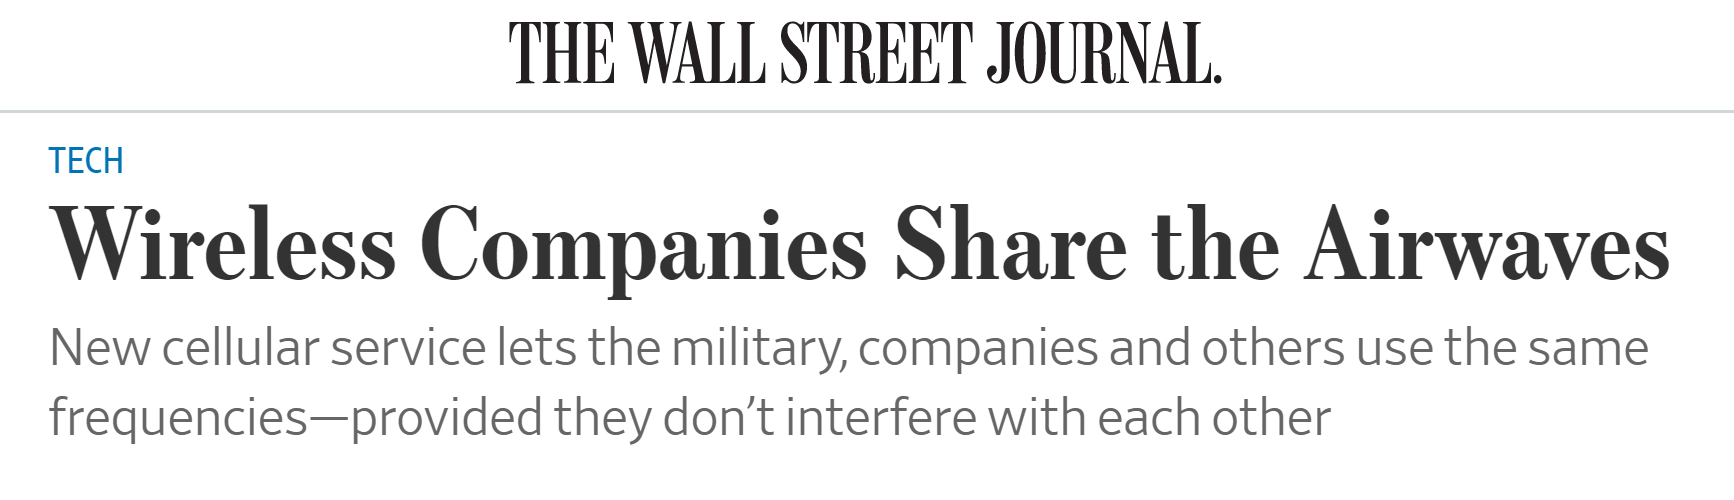
\includegraphics[width = 0.6\textwidth]{WSJ_1.PNG}
    \label{fig:1}
\end{figure}
\begin{figure}
    \centering
    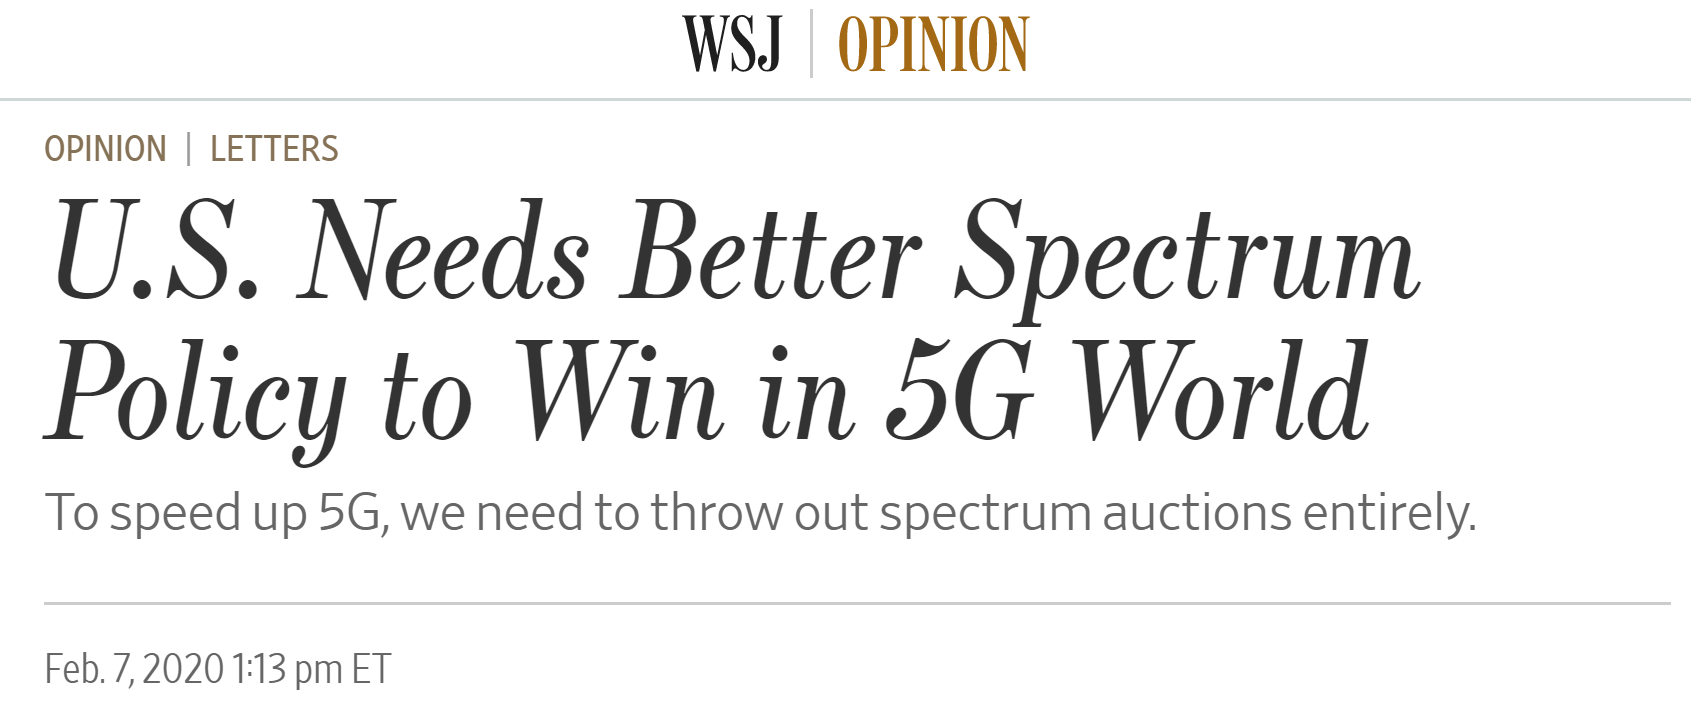
\includegraphics[width = 0.6\textwidth]{WSJ_2.PNG}
    \label{fig:1}
\end{figure}
\begin{figure}
    \centering
    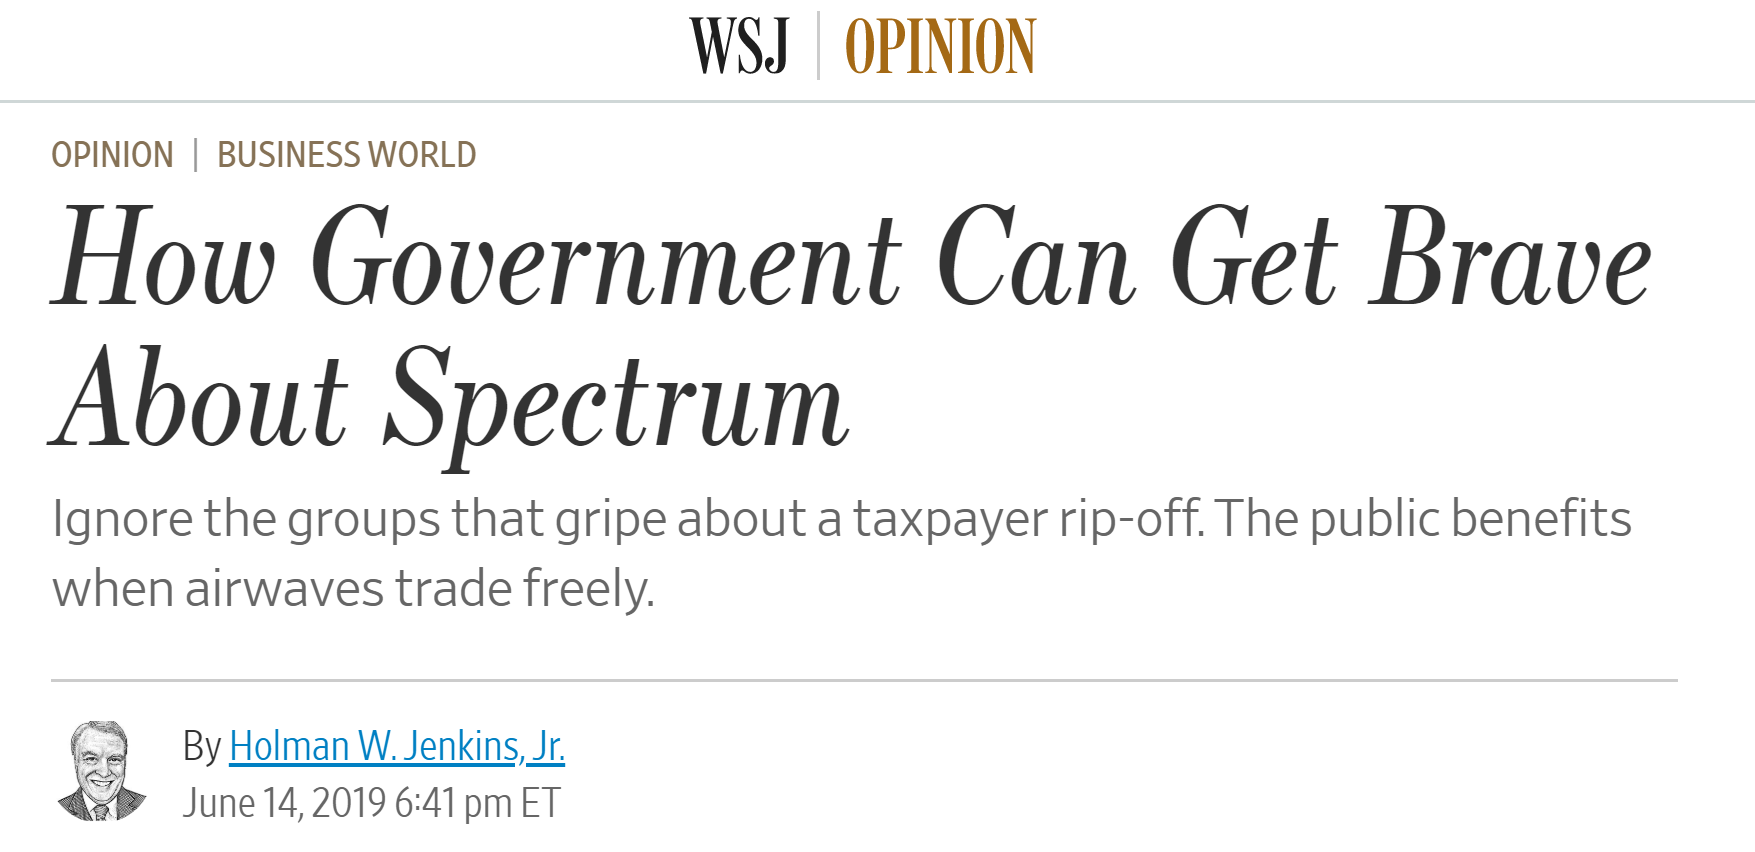
\includegraphics[width = 0.6\textwidth]{WSJ_3.PNG}
    \label{fig:1}
\end{figure}
\end{frame}
\begin{frame}{Motivation (2/2)}
\begin{figure}
    \centering
    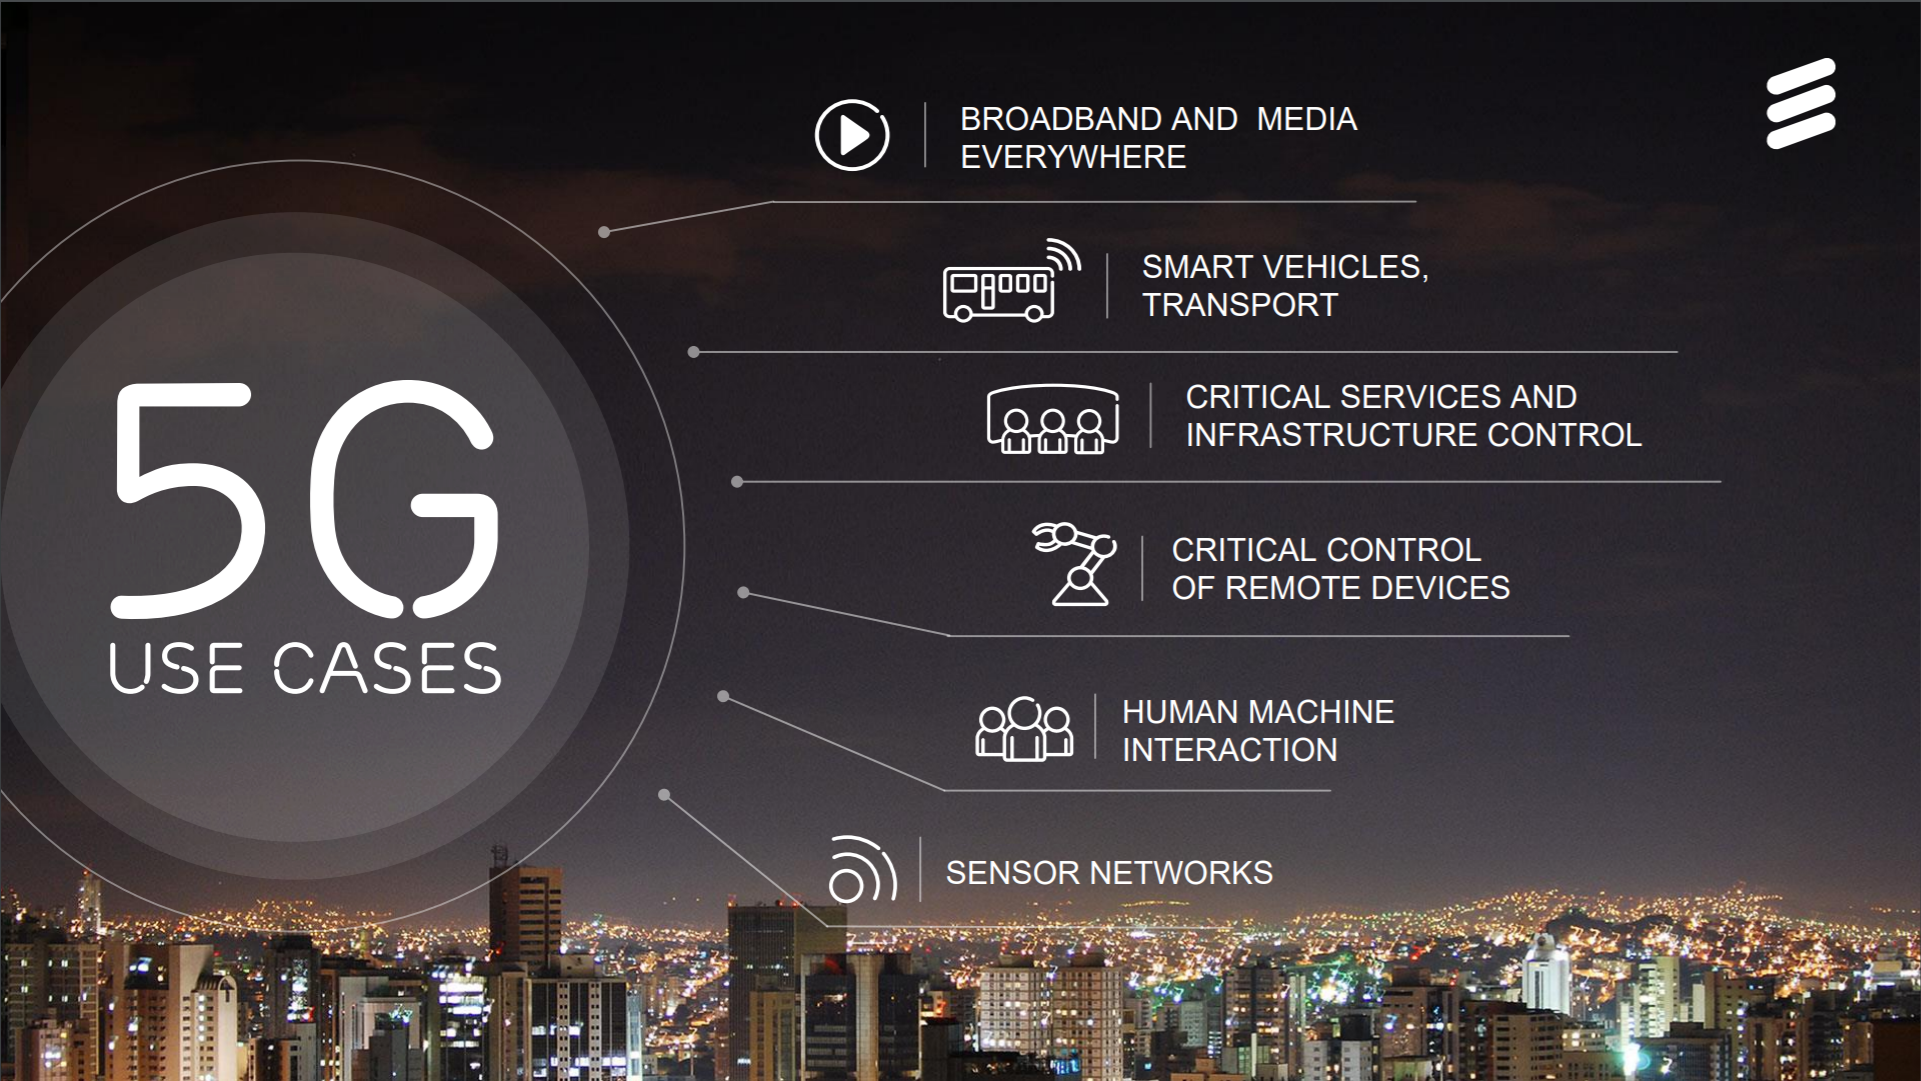
\includegraphics[width = 0.6\textwidth]{Ericsson.PNG}
    \label{fig:1}
\end{figure}
\begin{figure}
    \centering
    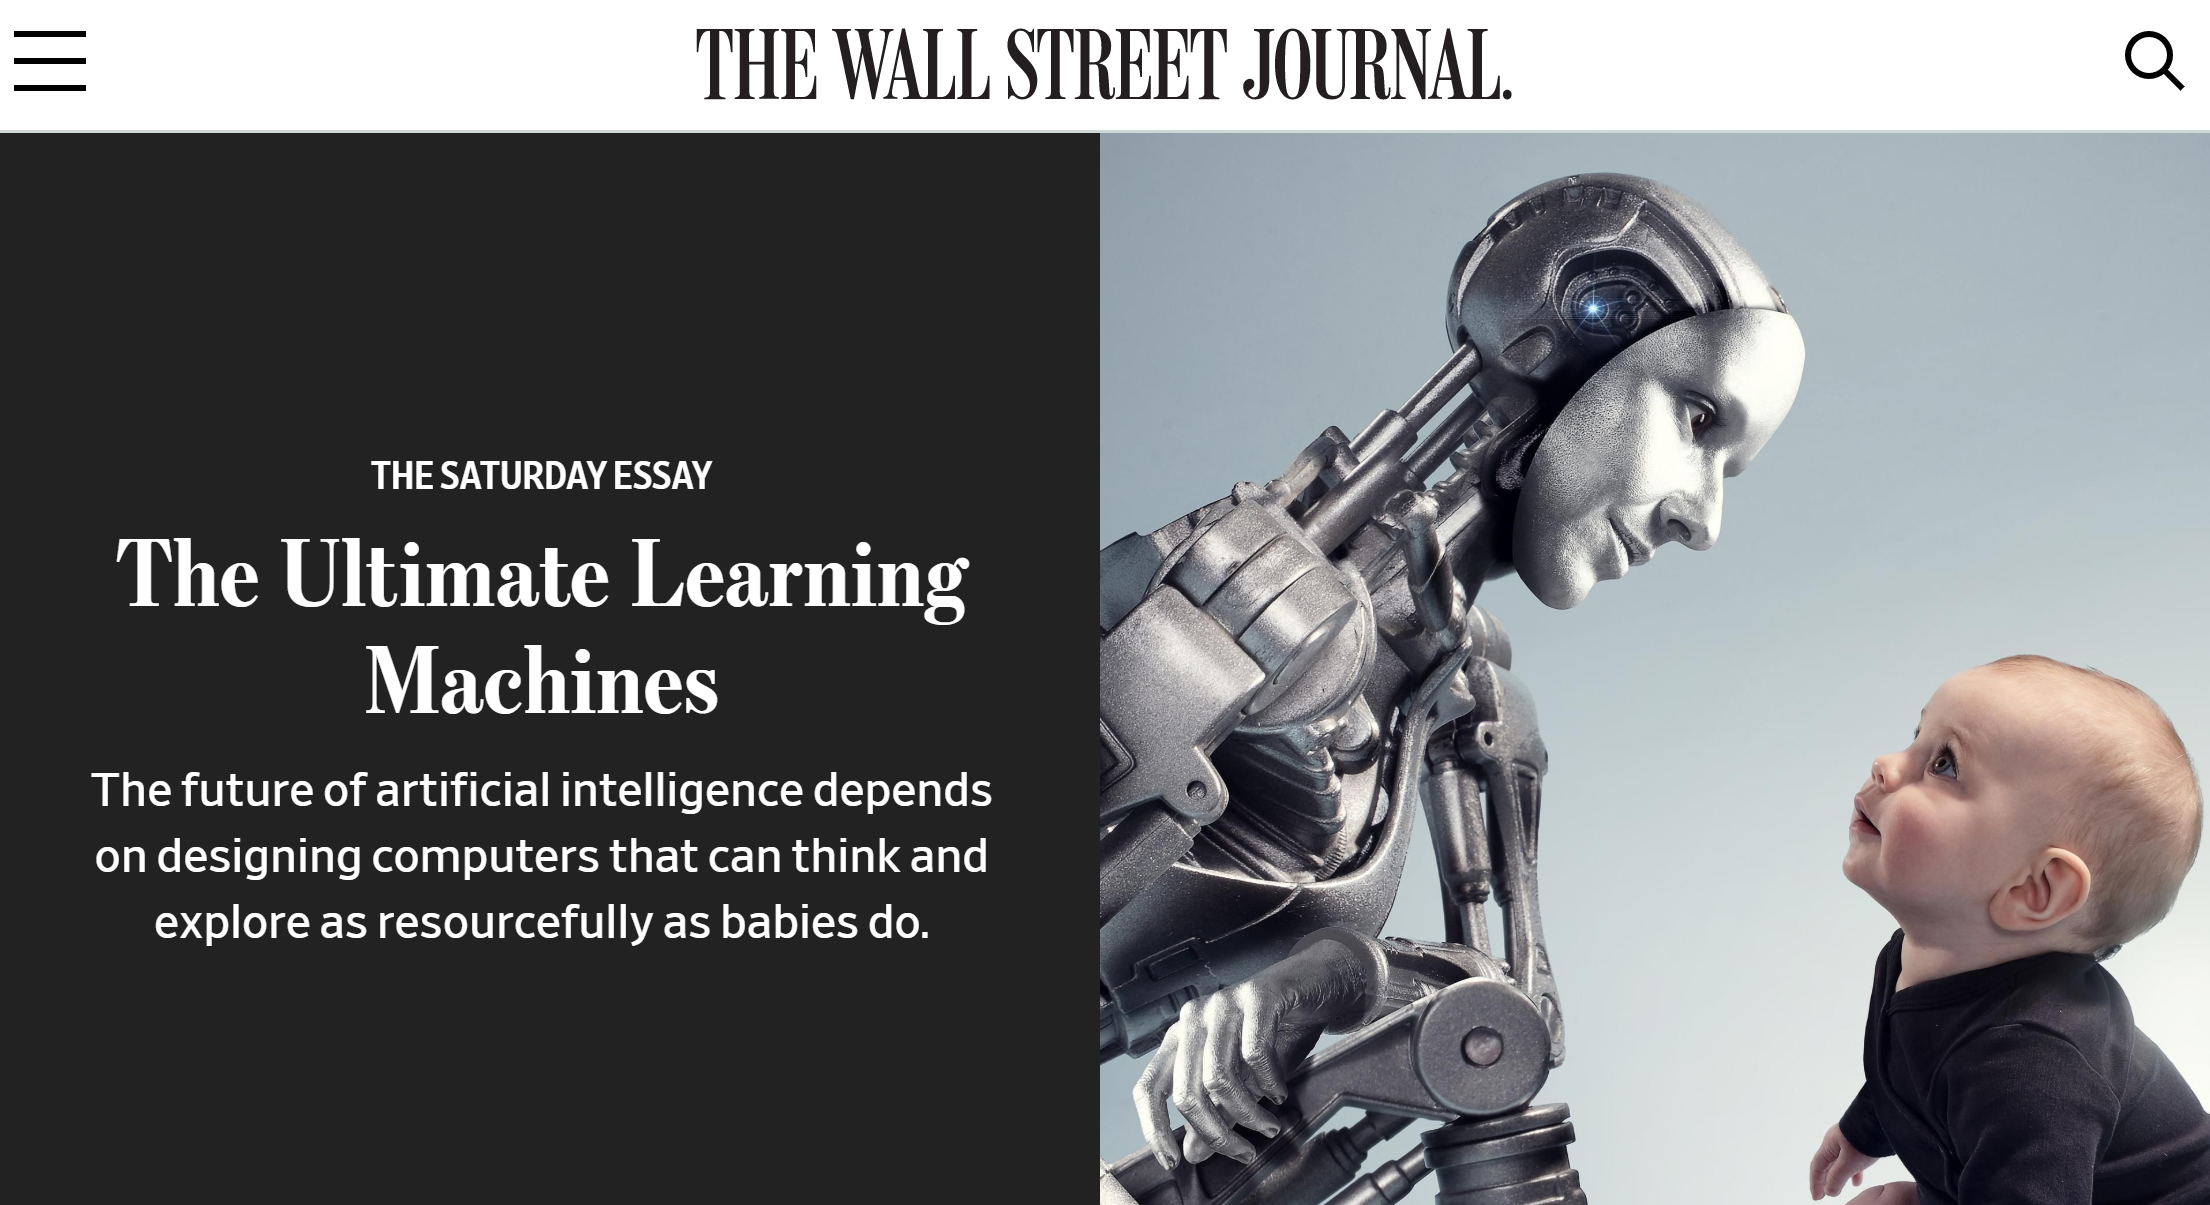
\includegraphics[width = 0.6\textwidth]{WSJ_4.PNG}
    \label{fig:1}
\end{figure}
\end{frame}
\begin{frame}{DARPA SC$2$: Problem Statement}
\begin{columns}[T]
\begin{column}{0.55\textwidth}
\color{blue}\rule{\linewidth}{4pt}
\begin{itemize}
    \item Multi-agent resource allocation
    \item Centralized setting
    \item Incumbents and Competitors
    \item Max our network's scores
    \item Ensure min mandated performance of ensemble
\end{itemize}
\end{column}%
\hfill%
\begin{column}{0.65\textwidth}
\color{magenta}\rule{\linewidth}{4pt}
\begin{figure}
    \centering
    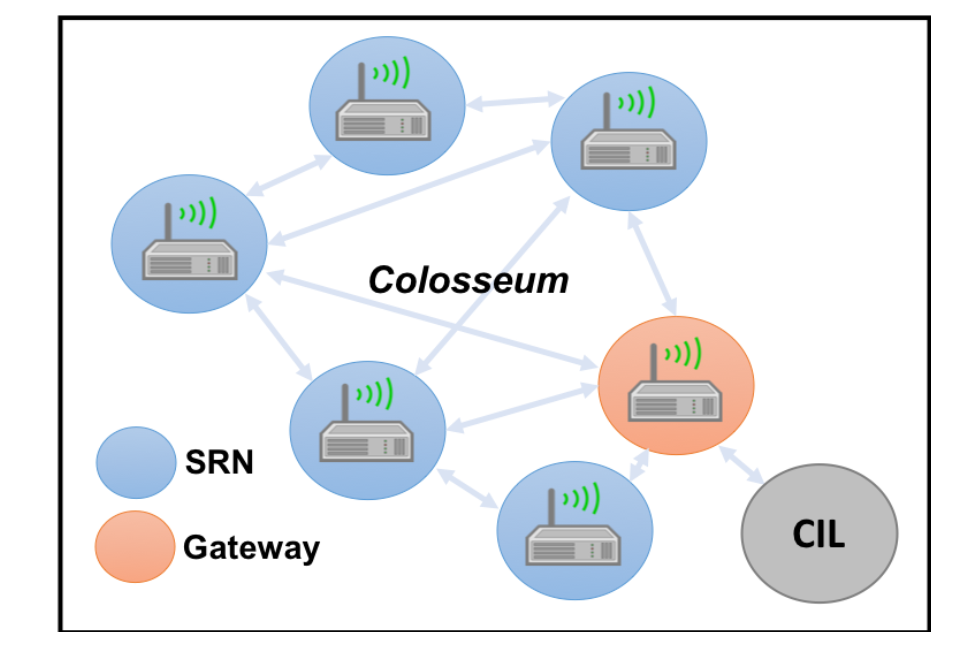
\includegraphics[width = 0.95\textwidth]{BAM!_Wireless_Architecture.PNG}
    \caption{The CIRN architecture}
    \label{fig:1}
\end{figure}
\end{column}%
\end{columns}
\end{frame}
\begin{frame}{Related Work: DARPA SC$2$ Competitors}
\begin{itemize}
      \item \textcolor{blue}{SCATTER}\footnote{\tiny{Giannoulis, et. al., ``The SCATTER approach...", 2019 IEEE DySPAN}}: OFDM waveform, McF-TDMA, Distributed channel allocation, Target-score based flow scheduling
      \item \textcolor{blue}{Zylinium}\footnote{\tiny{R.J. Baxley, R.S. Thompson, ``Team Zylinium...", 2019 IEEE DySPAN}}: OFDM PHY, CIL-based centralized channel allocation, Mixed integer programming for flow scheduling
\end{itemize}
\end{frame}
\begin{frame}{Challenges: Our Design Principles}
\begin{figure}
    \centering
    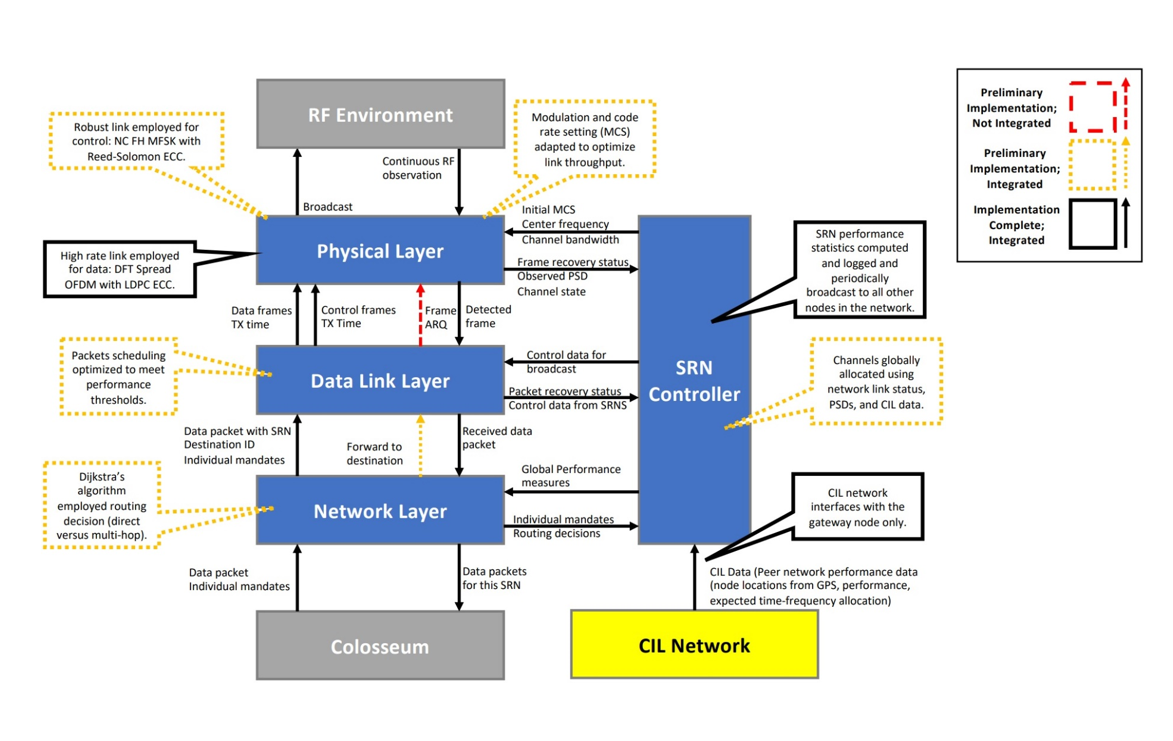
\includegraphics[width = 1.0\textwidth]{Layer-wise-design.PNG}
    \caption{Our radio's \textcolor{magenta}{network protocol stack}\footnote{\tiny{Contributions: DLL, Scoring, PSD${+}$Collab, CIL, GUI}}}
    \label{fig:1}
\end{figure}
\end{frame}
\begin{frame}{PHY: Transmission Power Control (1/3)}
    \begin{itemize}
        \item Collaborate to ensure incumbent interference compliance
        \item \textcolor{red}{Violation}: Aggregate interference at the incumbent exceeds current threshold
        \item \textcolor{cyan}{Reduce Tx power} of all SRNs proportionate to the excess interference divided by number of SRNs
    \end{itemize}
\end{frame}
\begin{frame}{PHY: Transmission Power Control (2/3)}
\begin{figure}
    \centering
    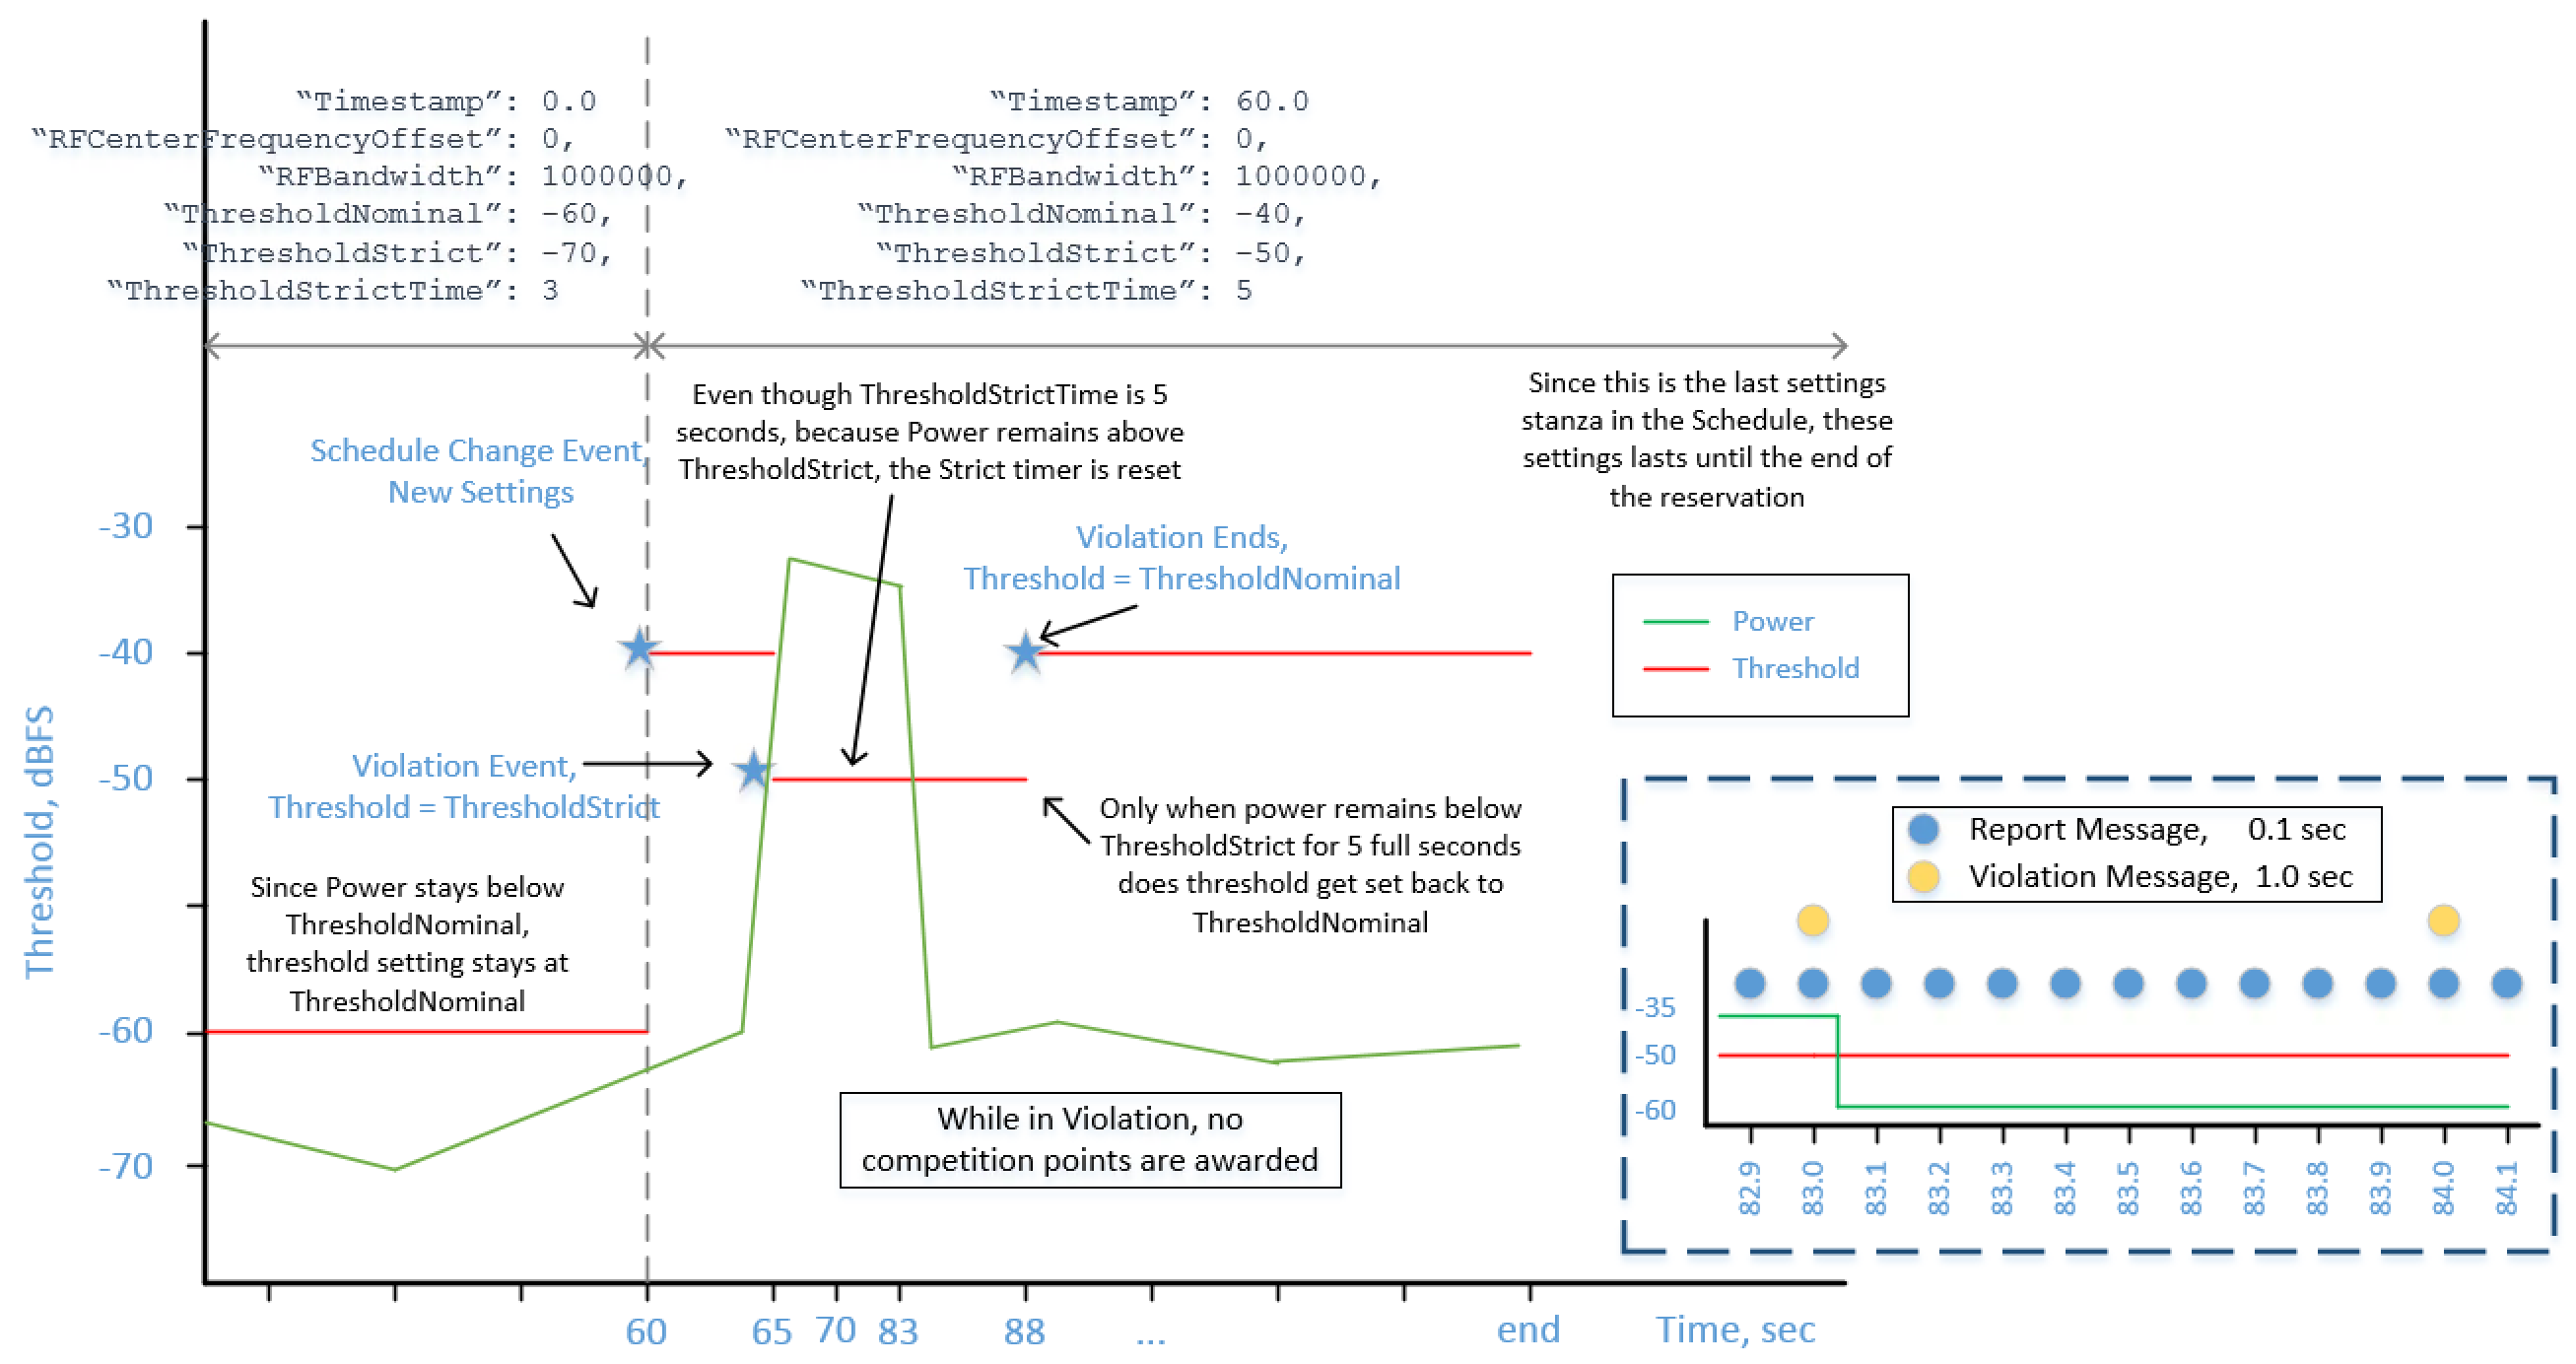
\includegraphics[width = 0.95\textwidth]{Passive_Incumbent.jpg}
    \caption{The temporal behavior of the \textcolor{magenta}{ Passive Incumbent}\footnote{\tiny{DARPA Colosseum}}}
    \label{fig:2}
\end{figure}
\end{frame}
\begin{frame}{PHY: Transmission Power Control (3/3)}
\begin{figure}
    \centering
    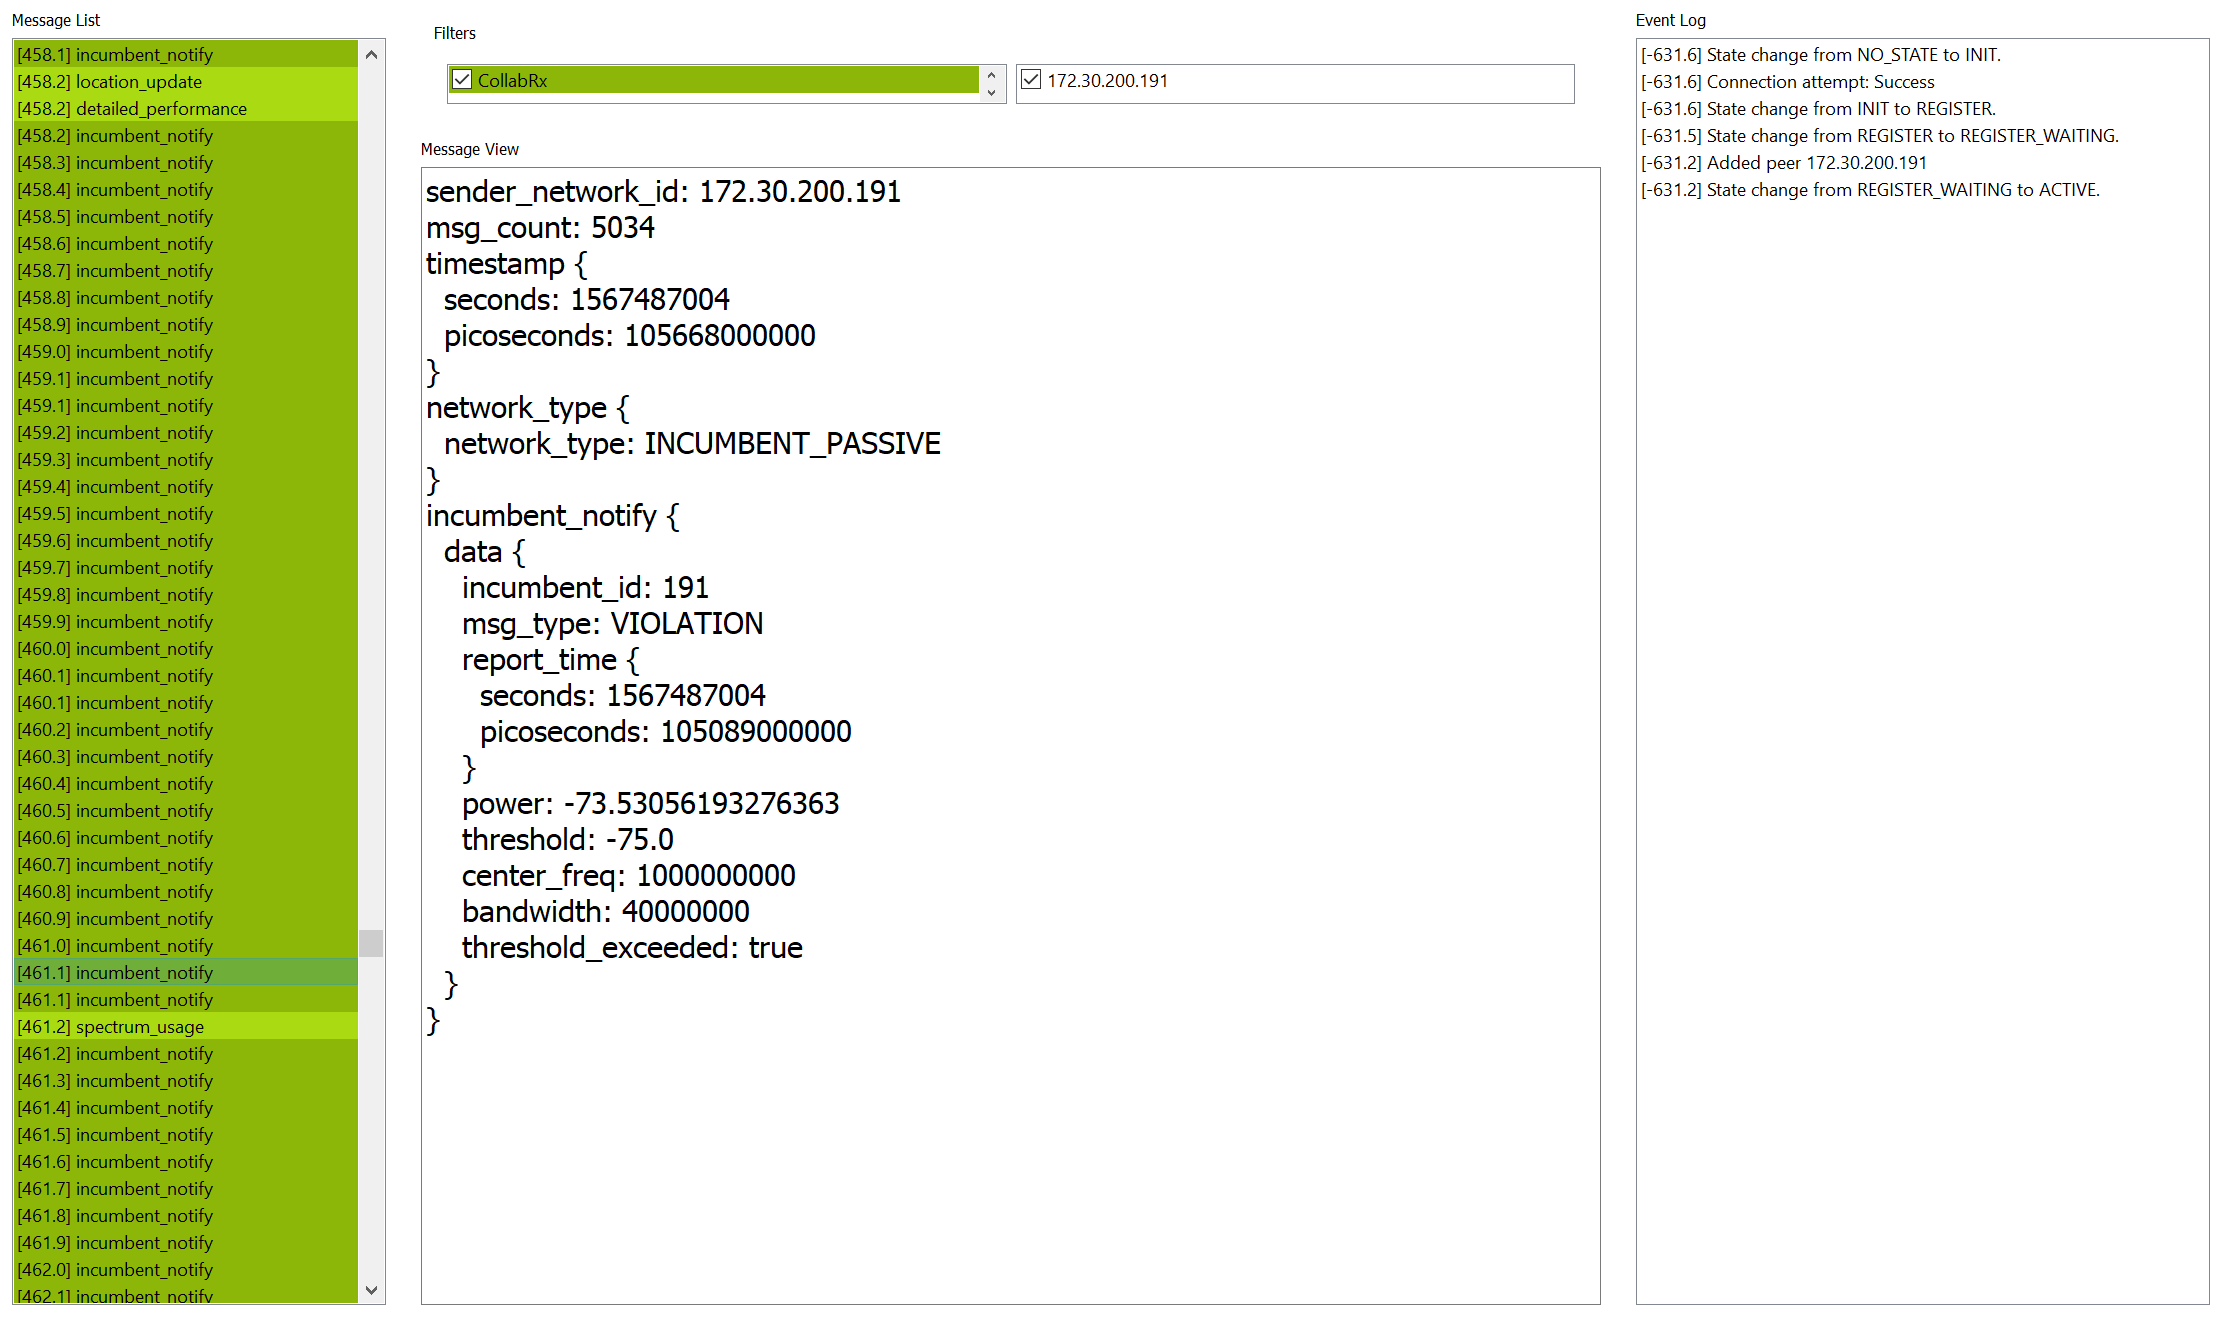
\includegraphics[width = 0.95\textwidth]{Passive_Incumbent_1.jpg}
    \caption{A \textcolor{red}{Violation} collaboration message from the Passive Incumbent}
    \label{fig:3}
\end{figure}
\end{frame}
\begin{frame}{PHY: The FSK Control Channel (1/2)}
    \begin{itemize}
        \item Short control frames
        \item Initial node discovery; Fallback link
        \item Non-coherent $8$-FSK link with $480$kHz of bandwidth
        \item Slotted ALOHA (without CD and backoff)
    \end{itemize}
\end{frame}
\begin{frame}{PHY: The FSK Control Channel (2/2)}
\begin{figure}
    \centering
    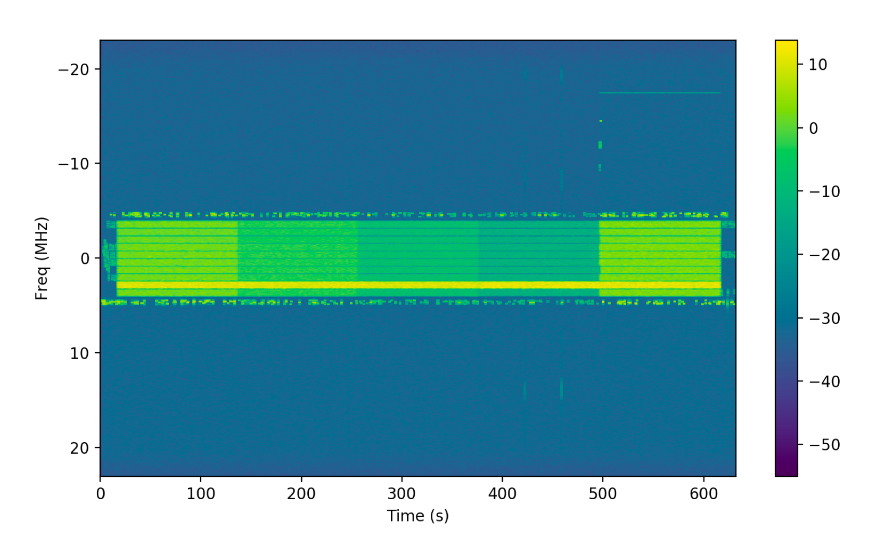
\includegraphics[width = 0.95\textwidth]{Control_Channels_At_Band_Edges.PNG}
    \caption{The center frequency \textcolor{magenta}{switches between the upper and lower spectral band-edges} during an SC$2$ Qual scenario}
    \label{fig:5}
\end{figure}
\end{frame}
\begin{frame}{PHY: The DFT-s-OFDM Data Channel (1/2)}
    \begin{itemize}
        \item Long control frames${+}$traffic
        \item $128$ sub-carriers: $108$ for data, $12$ for pilot, $8$ for null transmissions
        \item Allowed modulation: QPSK, QAM$16$, QAM$32$, and QAM$64$
        \item Allowed code rates: $\frac{1}{2}$, $\frac{2}{3}$, $\frac{3}{4}$, and $\frac{5}{6}$ (IEEE 802.11 QC-LDPC)
    \end{itemize}
\end{frame}
\begin{frame}{PHY: The DFT-s-OFDM Data Channel (2/2)}
\begin{figure}
    \centering
    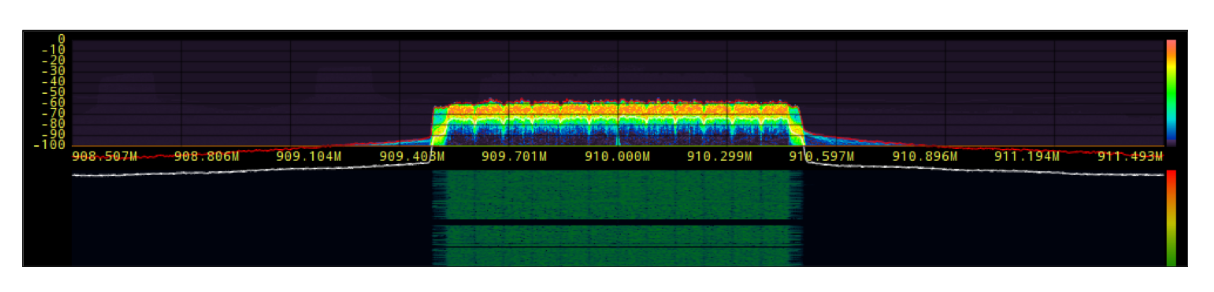
\includegraphics[width = 1.0\textwidth]{Data_Channel_DFT-spread-OFDM_Power_Spectrum.PNG}
    \caption{The \textcolor{magenta}{power spectrum} of DFT-s-OFDM waveform}
    \label{fig:6}
\end{figure}
\end{frame}
\begin{frame}{PHY: MCS Adaptation (1/3)}
\begin{figure}
    \centering
    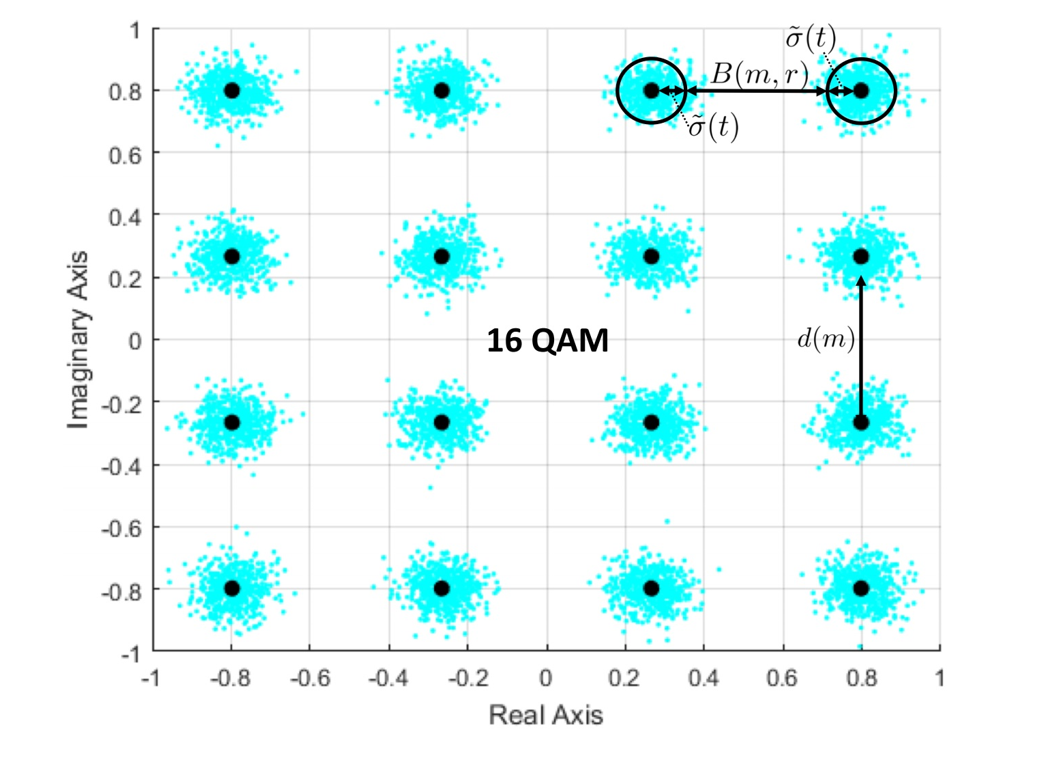
\includegraphics[width = 0.85\textwidth]{MCS_Constellation_Diagram.PNG}
    \caption{The MCS adaptation algorithm based on \textcolor{magenta}{minimizing the distance} between the circles centered at two adjacent constellation symbols}
    \label{fig:7}
\end{figure}
\end{frame}
\begin{frame}{PHY: MCS Adaptation (2/3)}
\begin{figure}
    \centering
    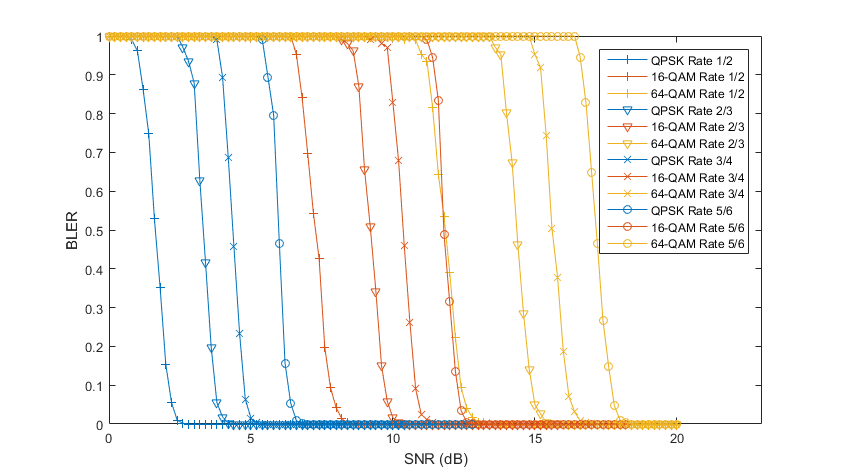
\includegraphics[width = 0.95\textwidth]{BLER.png}
    \caption{Simulated \textcolor{magenta}{BLER} curves for different combinations of modulation order and code rate}
    \label{fig:8}
\end{figure}
\end{frame}
\begin{frame}{PHY: MCS Adaptation (3/3)}
\begin{figure}
    \centering
    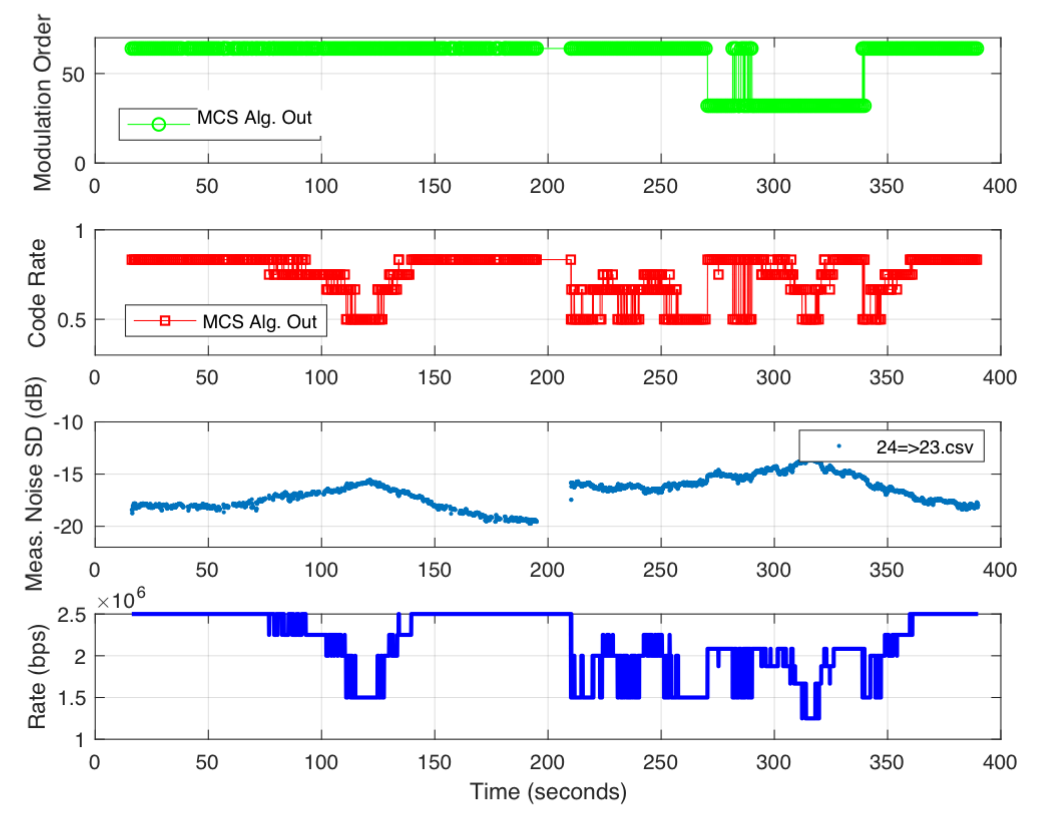
\includegraphics[width = 0.75\textwidth]{Payline_MCS_Adaptation.PNG}
    \caption{\textcolor{magenta}{MCS adaptation to changes in noise variance} during an SC$2$ Payline scenario}
    \label{fig:9}
\end{figure}
\end{frame}
\begin{frame}{DLL: Prioritized Flow Scheduling with ARQ (1/4)}
    \begin{itemize}
        \item VOIP${=}4$, UAV CCTV stream${=}9$, Video bombing run${=}15$ 
        \item Find the UB and LB of a QS using flow info and link quality
        \item Rank the flows in the decreasing order of their \textcolor{magenta}{value/resource}
        \item Fit into the QS in the ranked order w/ \textcolor{magenta}{recursive revisitation}
    \end{itemize}
\end{frame}
\begin{frame}{DLL: Prioritized Flow Scheduling with ARQ (2/4)}
\begin{figure}
    \centering
    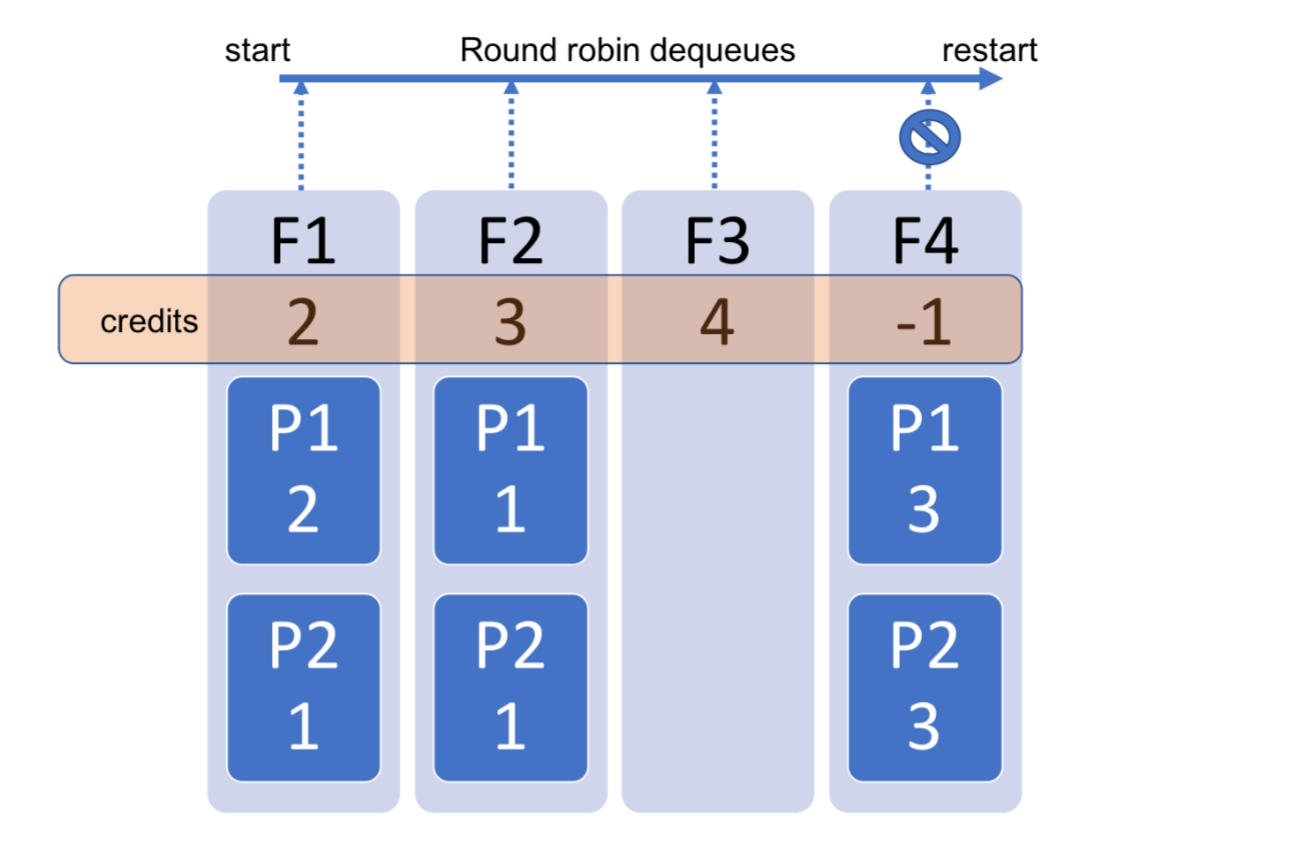
\includegraphics[width = 0.95\textwidth]{Deficit_Round_Robin_Scheduling.PNG}
    \caption{\textcolor{magenta}{Deficit round-robin scheduling} with a concept of ``credits"}
    \label{fig:11}
\end{figure}
\end{frame}
\begin{frame}{DLL: Prioritized Flow Scheduling with ARQ (3/4)}
\begin{figure}
    \centering
    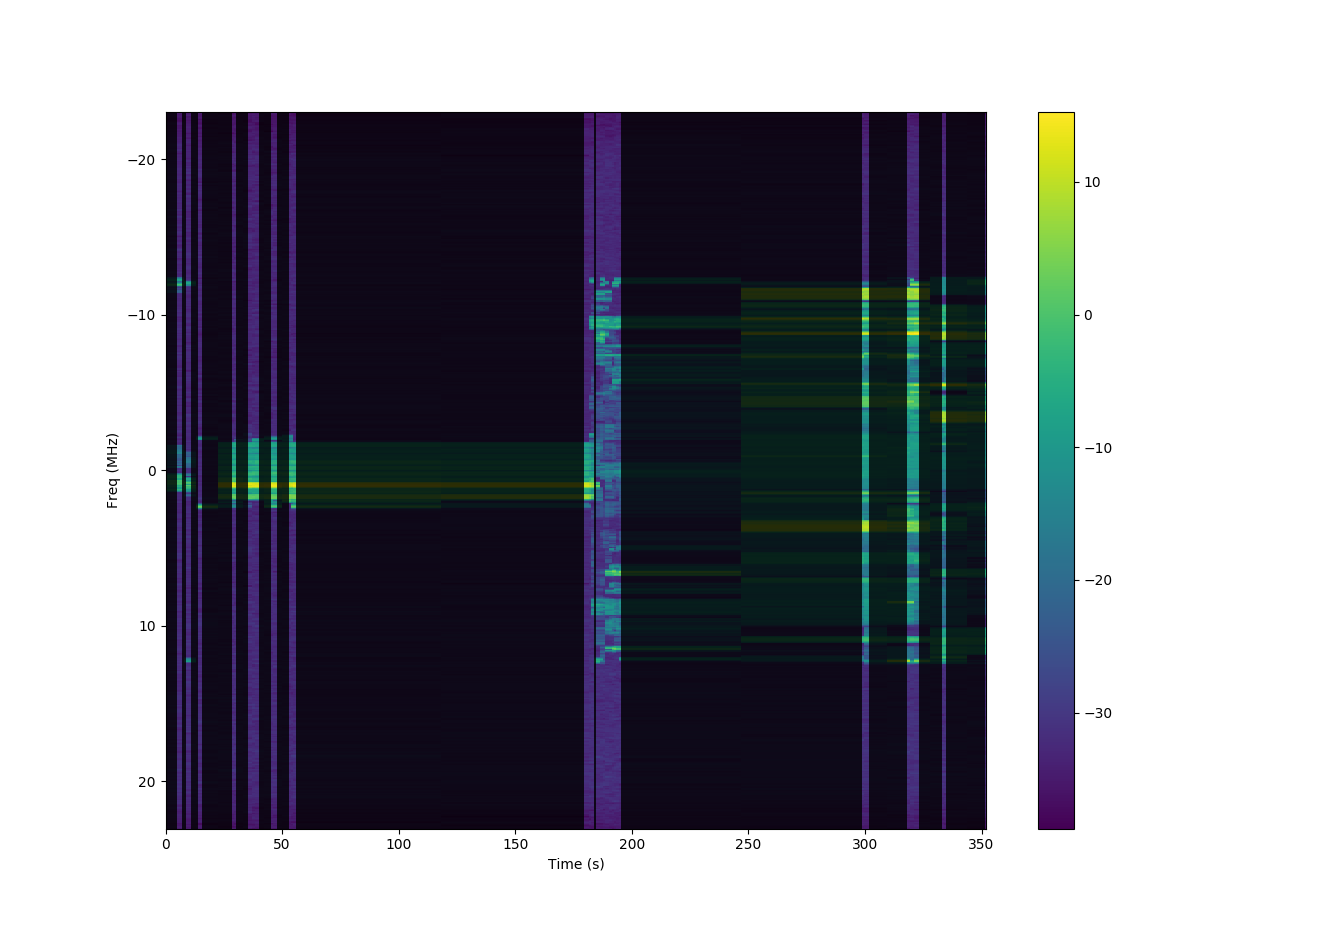
\includegraphics[width = 0.85\textwidth]{PSD_without_fix_payline.png}
    \caption{A situation in which PSD flows from an SRN (to the GW) are \textcolor{blue}{not prioritized} over other flows during an SC$2$ Payline scenario}
    \label{fig:12}
\end{figure}
\end{frame}
\begin{frame}{DLL: Prioritized Flow Scheduling with ARQ (4/4)}
\begin{figure}
    \centering
    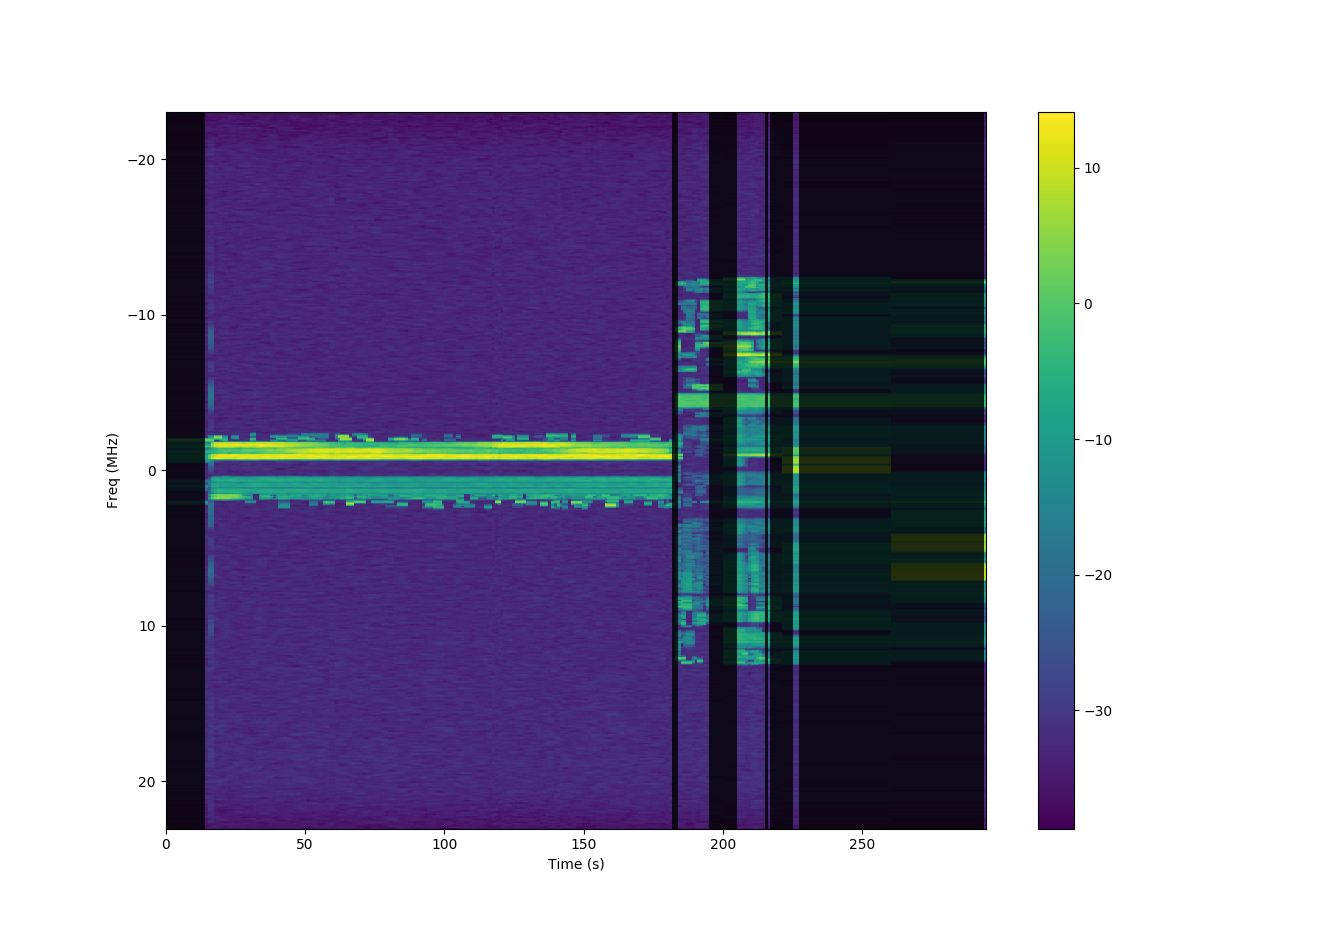
\includegraphics[width = 0.85\textwidth]{PSD_with_fix_payline.png}
    \caption{A situation in which PSD flows from an SRN (to the GW) are \textcolor{blue}{prioritized} over most other flows during an SC$2$ Payline scenario: \textcolor{red}{leads to a drop in scores}}
    \label{fig:13}
\end{figure}
\end{frame}
\begin{frame}{MAC: BW and Channel Allocation (1/3)}
\begin{itemize}
        \item \textcolor{blue}{BW}: Traffic stats, QoS reqs, link quality, self \& peer scores
        \item \textcolor{blue}{$f_{c}$}: PSD obs, self \& peer scores, GPS, Tx power
        \item A heuristic search to determine the center frequencies that minimize the interference at our SRN receivers
\end{itemize}
\end{frame}
\begin{frame}{MAC: BW and Channel Allocation (2/3)}
\begin{figure}
    \centering
    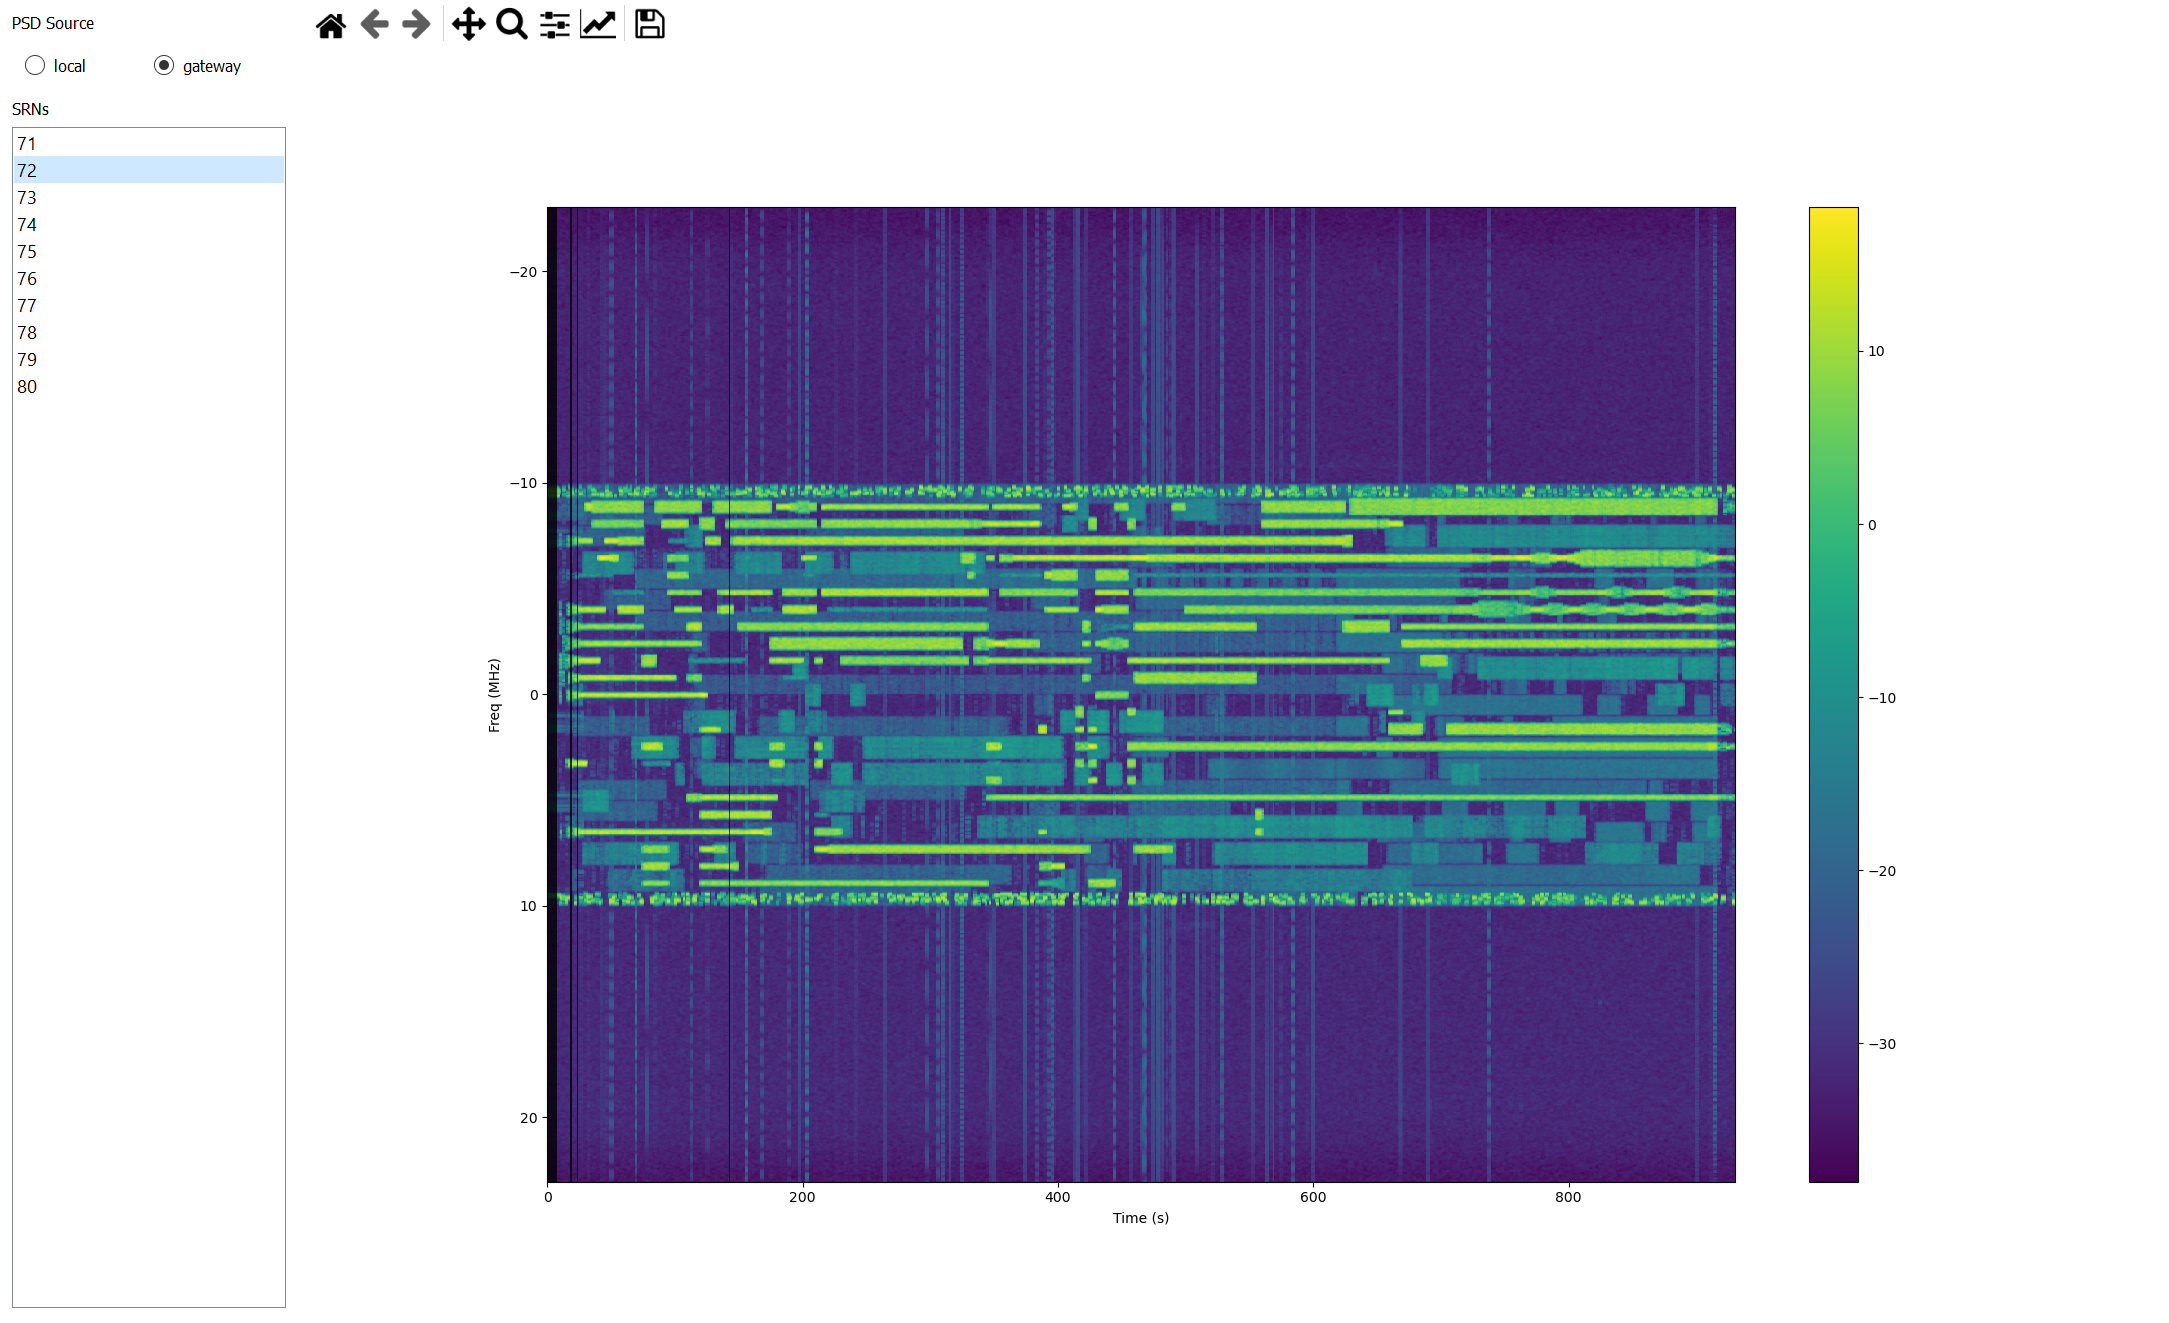
\includegraphics[width = 0.95\textwidth]{Alleys_PSD.PNG}
    \caption{The PSD observations \textcolor{magenta}{from SRN $72$ to our GW} during an SC$2$ Alleys of Austin scenario}
    \label{fig:15}
\end{figure}
\end{frame}
\begin{frame}{MAC: BW and Channel Allocation (3/3)}
\begin{figure}
    \centering
    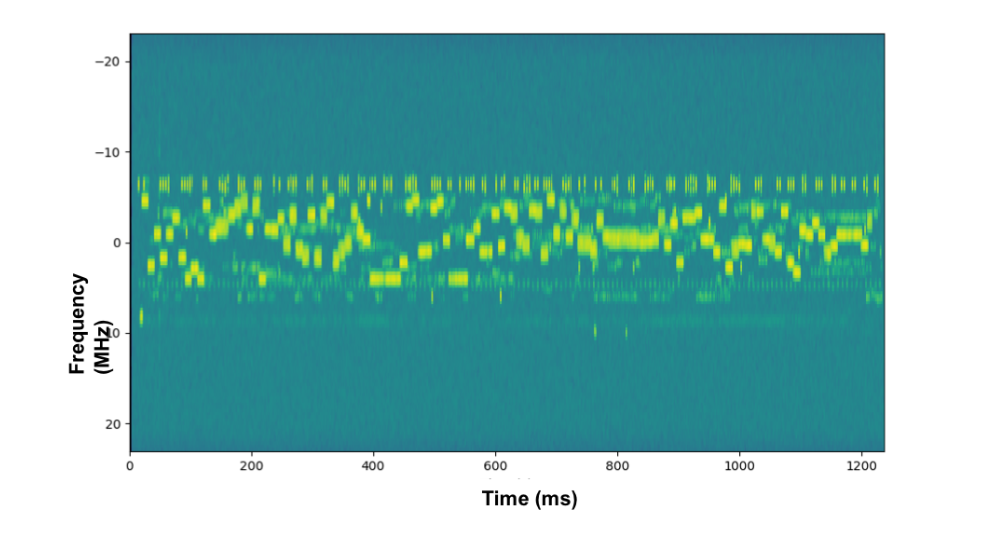
\includegraphics[width = 0.95\textwidth]{Alleys_of_Austin_Channel_Access.PNG}
    \caption{The spectrum occupied by our SRNs (time-frequency map) with \textcolor{magenta}{re-allocations dictated by a combination of local PSD obs and CIL msgs}, during an SC$2$ Alleys of Austin scenario}
    \label{fig:14}
\end{figure}
\end{frame}
\begin{frame}{NET: Multi-hop Routing (1/3)}
Binary link status vectors$\rightarrow$Route tables$\rightarrow$Dijkstra's algorithm
\begin{figure}
    \centering
    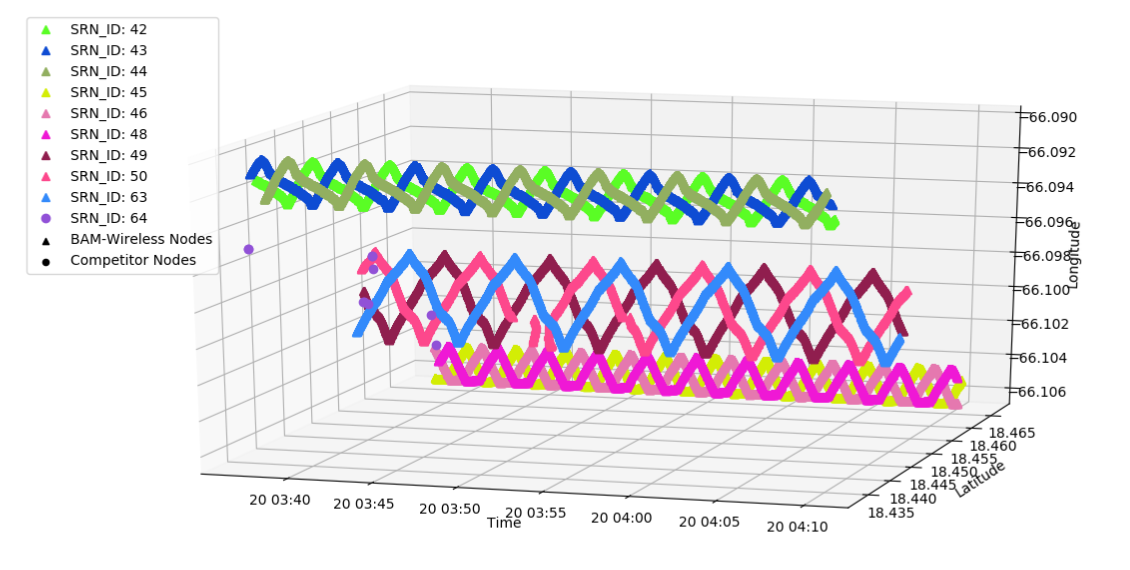
\includegraphics[width = 0.95\textwidth]{Payline_Node_GPS_Locations.PNG}
    \caption{\textcolor{magenta}{SRN mobility} as emulated in an SC$2$ Payline scenario causes variations in RF propagation characteristics}
    \label{fig:17}
\end{figure}
\end{frame}
\begin{frame}{NET: Multi-hop Routing (2/3)}
    \begin{figure}
    \centering
    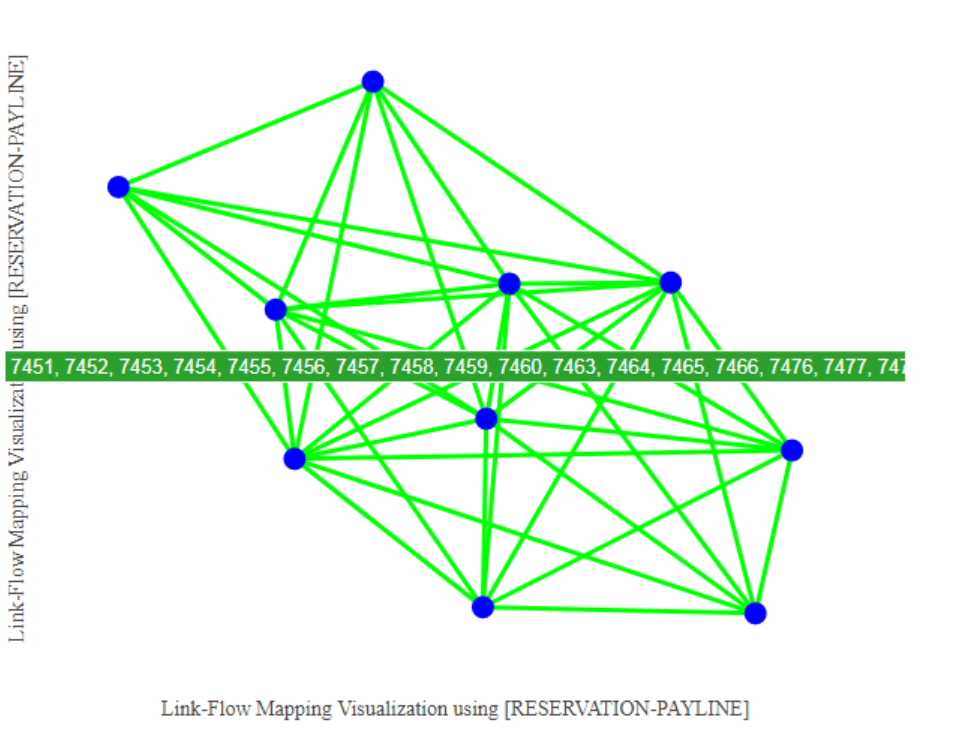
\includegraphics[width = 0.85\textwidth]{Network_Graph_Payline.PNG}
    \caption{Our \textcolor{magenta}{network map} in an SC$2$ Payline scenario}
    \label{fig:19}
\end{figure}
\end{frame}
\begin{frame}{NET: Multi-hop Routing (3/3)}
\begin{figure}
    \centering
    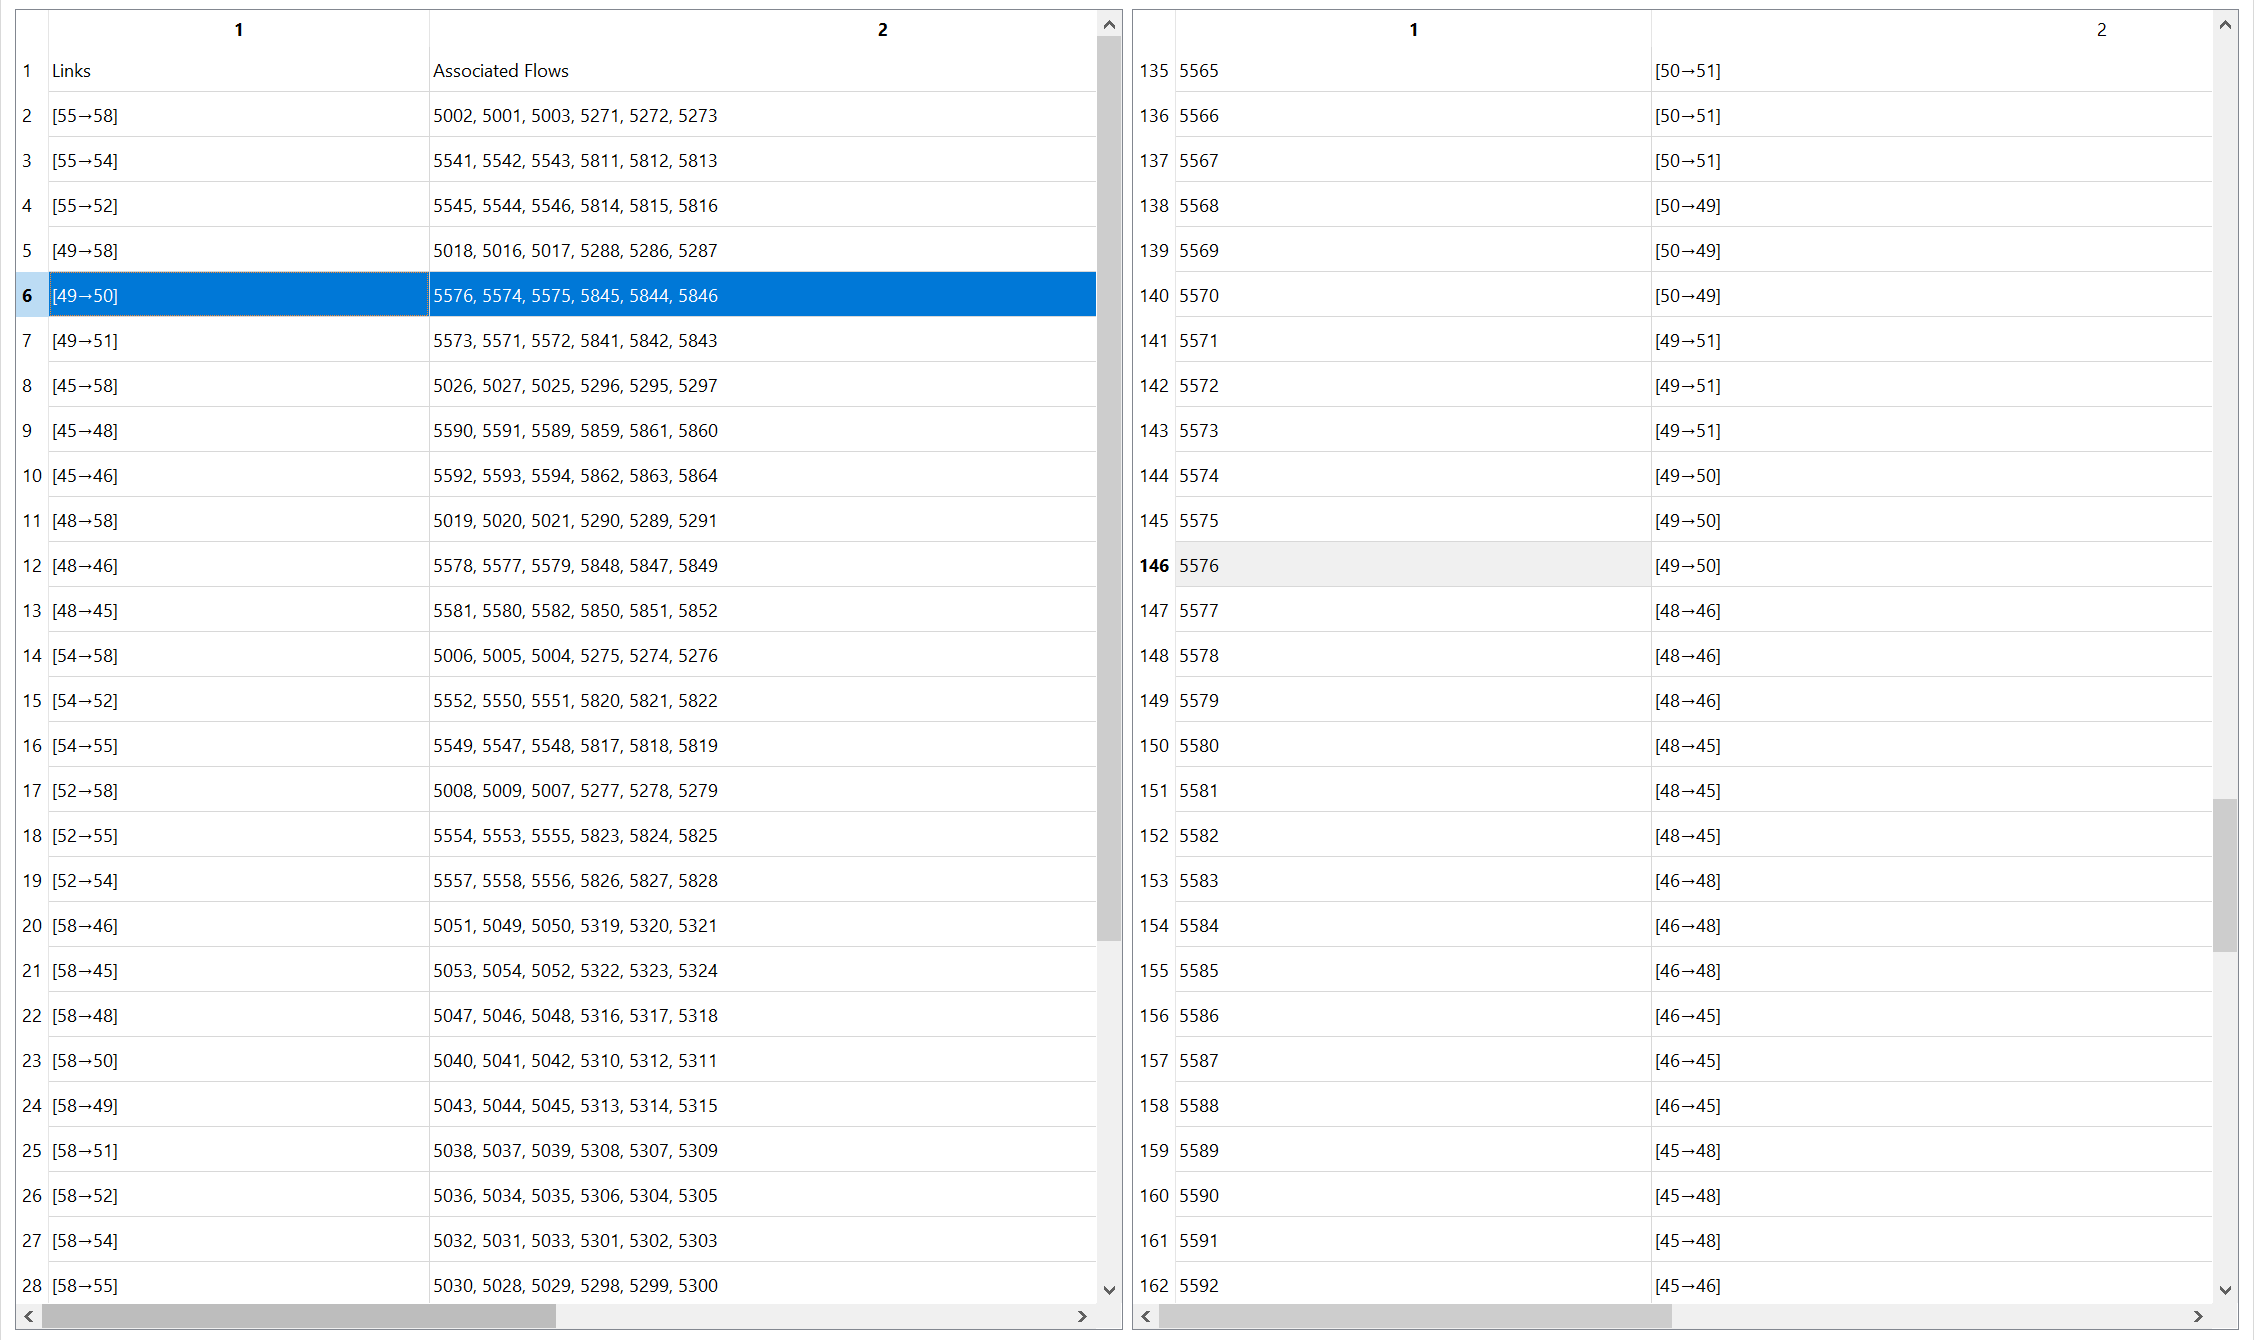
\includegraphics[width = 0.95\textwidth]{Link_Flow_Mapping.PNG}
    \caption{\textcolor{magenta}{Link-Flow Mapping} for our network in an SC$2$ Payline scenario}
    \label{fig:18}
\end{figure}
\end{frame}
\begin{frame}{SC$2$ Wildfire: Disaster-Relief Scenario Analysis}
    \begin{figure}
    \centering
    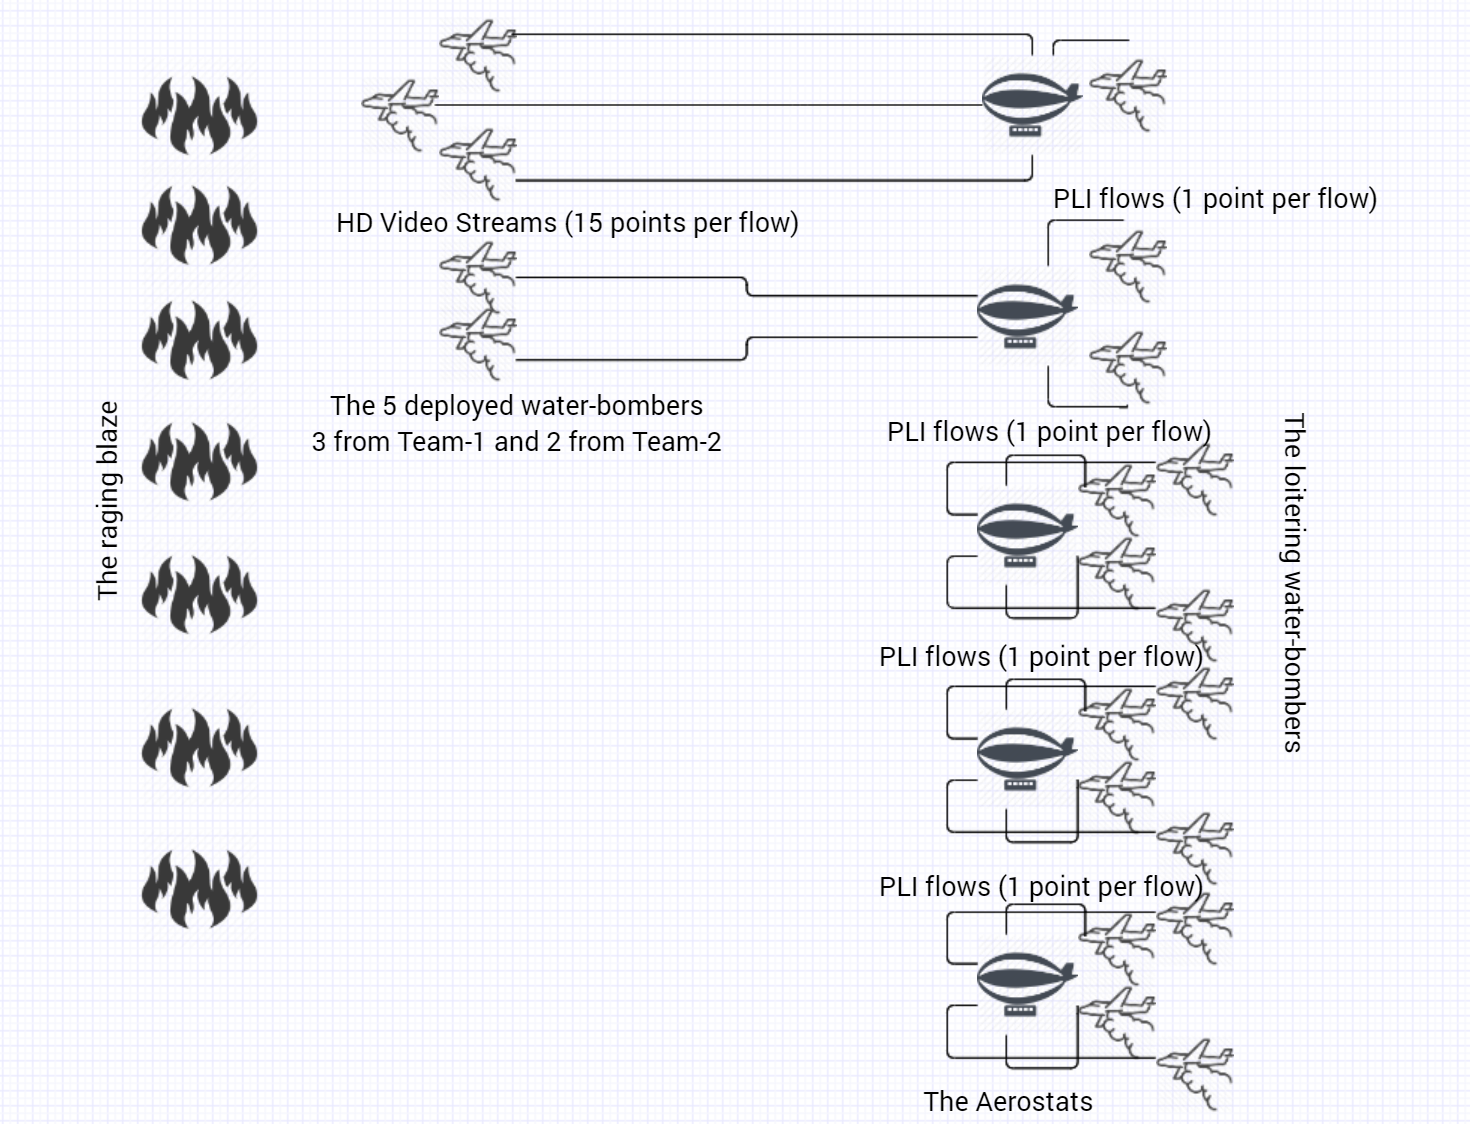
\includegraphics[width = 0.90\textwidth]{Wildfire_Deployment.PNG}
    \caption{The logistics of the SC$2$ Wildfire deployment scenario}
    \label{fig:18}
\end{figure}
\end{frame}
\begin{frame}{BAM! Wireless Network Performance Analysis: SC$2$ Wildfire (2/2)}
\begin{figure}
    \centering
    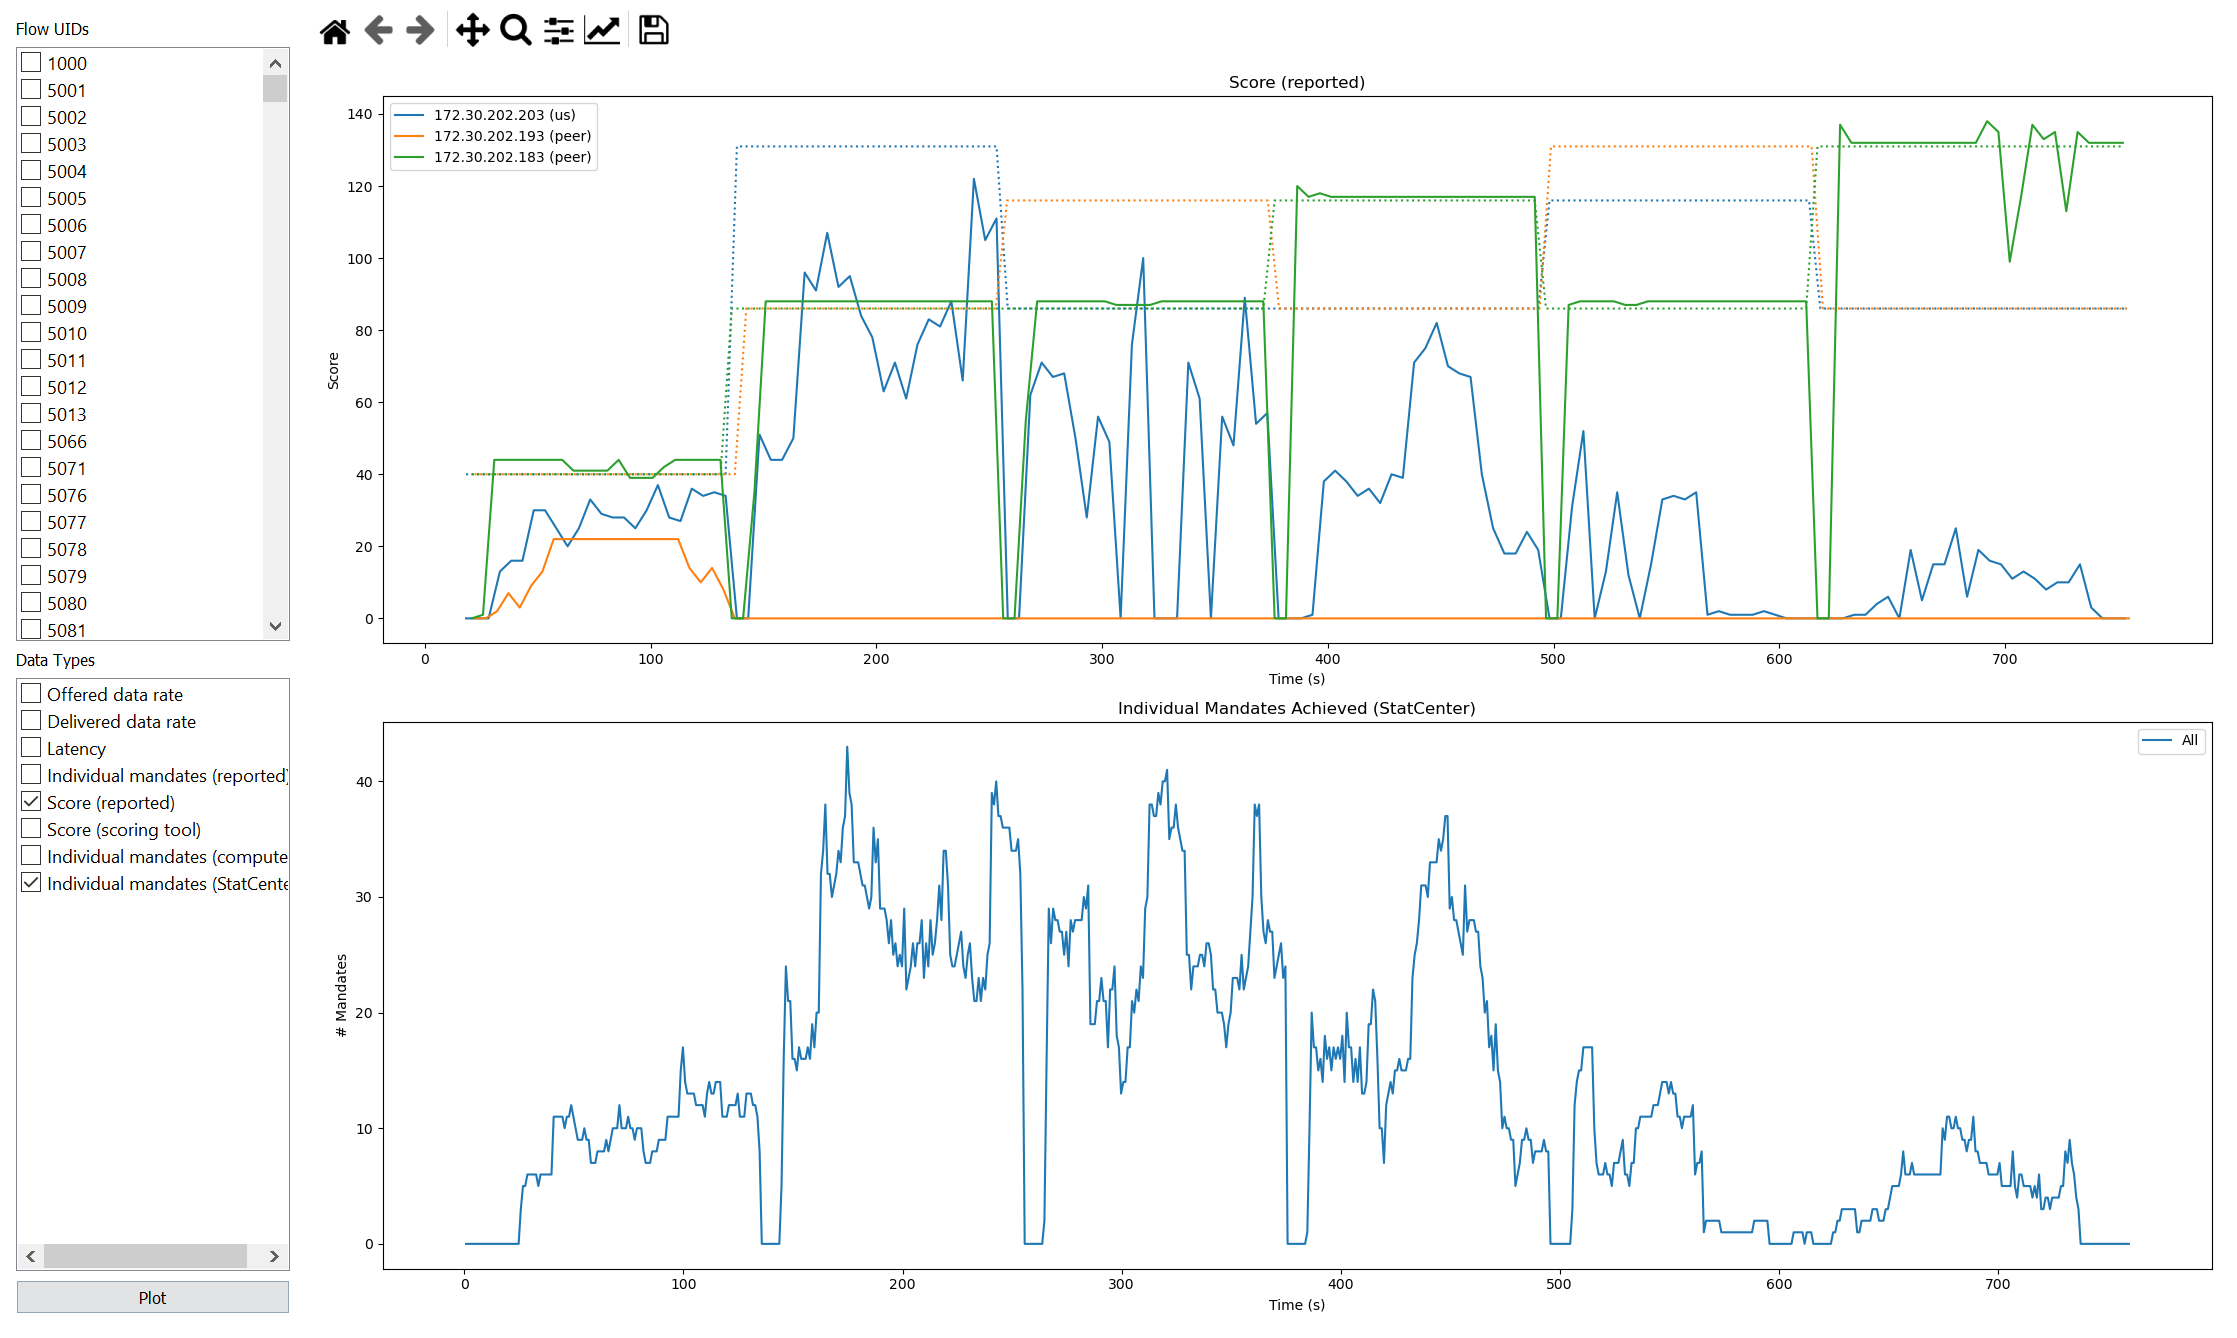
\includegraphics[width = 0.90\textwidth]{Wildfire_Scoring.PNG}
    \caption{The scores attained by our network: \textcolor{magenta}{much better} than the \textcolor{orange}{peer in orange} throughout, \textcolor{blue}{performance comparable} to the \textcolor{green}{peer in green} in Stages $1-3$}
    \label{fig:24}
\end{figure}
\end{frame}
\begin{frame}{Condensed Simplification: Spectrum Sensing \& Access}
\begin{itemize}
    \item Focus on spectrum sensing and access in the MAC
    \item Centralized deployment
    \item Simplified considerations that scale well to real scenarios
    \item \textcolor{magenta}{HMMs} and \textcolor{magenta}{Approx. POMDPs} to find optimal policy
\end{itemize}
\end{frame}
\begin{frame}{Related Work}
\begin{itemize}
  \item Custom heuristics\footnote{\label{F4}\tiny{M. Gao, et. al., ``Fast Spectrum Sensing...", 2014 IEEE MilCom}}, HMMs\footnote{\label{F6}\tiny{C. Park, et. al., ``HMM Based Channel Status Predictor for Cognitive Radio", 2007 APAC MW Conference}}, MABs\footnote{\label{F5}\tiny{K. Cohen, et. al., ``Restless Multi-Armed Bandits...", 2014 Asilomar}}, RL-agents\footnote{\label{F3}\tiny{J. Lund\'{e}n, et. al., ``Multiagent Spectrum Sensing...", IEEE Journal of Selected Topics in Signal Processing}}: \textcolor{red}{Issues}
  \begin{itemize}
      \item \textcolor{red}{Noise-free} [\ref{F4}] obs or \textcolor{red}{Ignored} [\ref{F3}] errors in state estimation
      \item \textcolor{red}{Failure to exploit} [\ref{F5}] time-frequency correlation structure
      \item \textcolor{red}{Apriori knowledge} [\ref{F3}] of this correlation model
      \item \textcolor{red}{Offline estimation} [\ref{F4}] of this correlation model
      \item \textcolor{red}{No support} ([\ref{F3}], [\ref{F4}]) for tuning throughput and interference
  \end{itemize}
\end{itemize}
\end{frame}
\begin{frame}{Challenges: Solutions\footnote{\tiny{B. Keshavamurthy, N. Michelusi, ``Spectrum Sensing in Cognitive Radio Networks via Approximate POMDP", Unpublished, 2020}}}
\begin{itemize}
    \item \textcolor{cyan}{Noisy} observation model with Rayleigh fading channels
    \item \textcolor{cyan}{Successfully exploit} time-frequency correlation structure
    \item \textcolor{cyan}{No apriori knowledge} of this correlation model
    \item \textcolor{cyan}{Online estimation} of this correlation model
    \item \textcolor{cyan}{Approximate POMDP with heuristics}
    \item \textcolor{cyan}{Support} for throughput and interference tuning
\end{itemize}
\end{frame}
\begin{frame}{Signal Model}
\footnotesize{\textcolor{magenta}{OFDMA}; \textcolor{magenta}{AWGN} observation model; \textcolor{magenta}{Rayleigh} fading channel}
    \begin{figure}
    \centering
    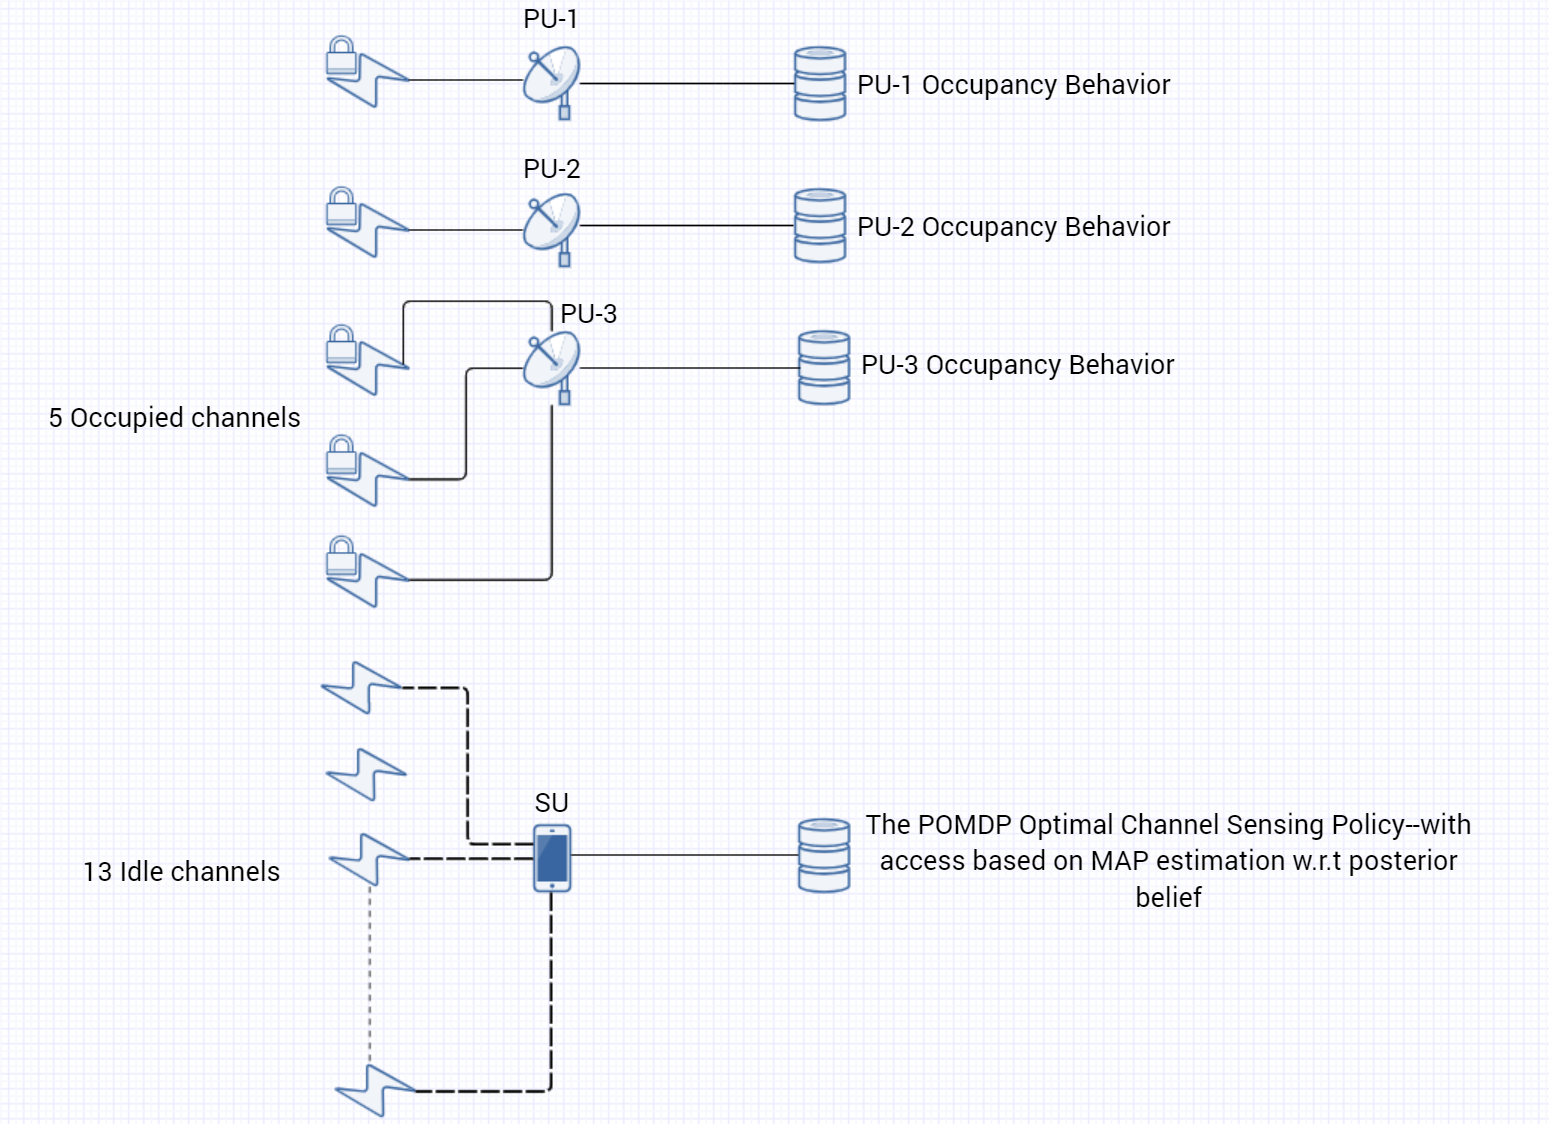
\includegraphics[width = 0.90\textwidth]{POMDP_Network.PNG}
    \caption{The simplified cognitive radio network under analysis}
    \label{fig:24}
\end{figure}
\end{frame}
\begin{frame}{PU Occupancy Model}
\footnotesize{\[\mathbb{P}(\vec{B}(i+1)|\vec{B}(i))=\mathbb{P}(B_{1}(i+1)|B_{1}(i))\prod_{k=2}^{K}\mathbb{P}(B_{k}(i+1)|B_{k}(i), B_{k-1}(i+1))\]}
\begin{figure}
    \centering
    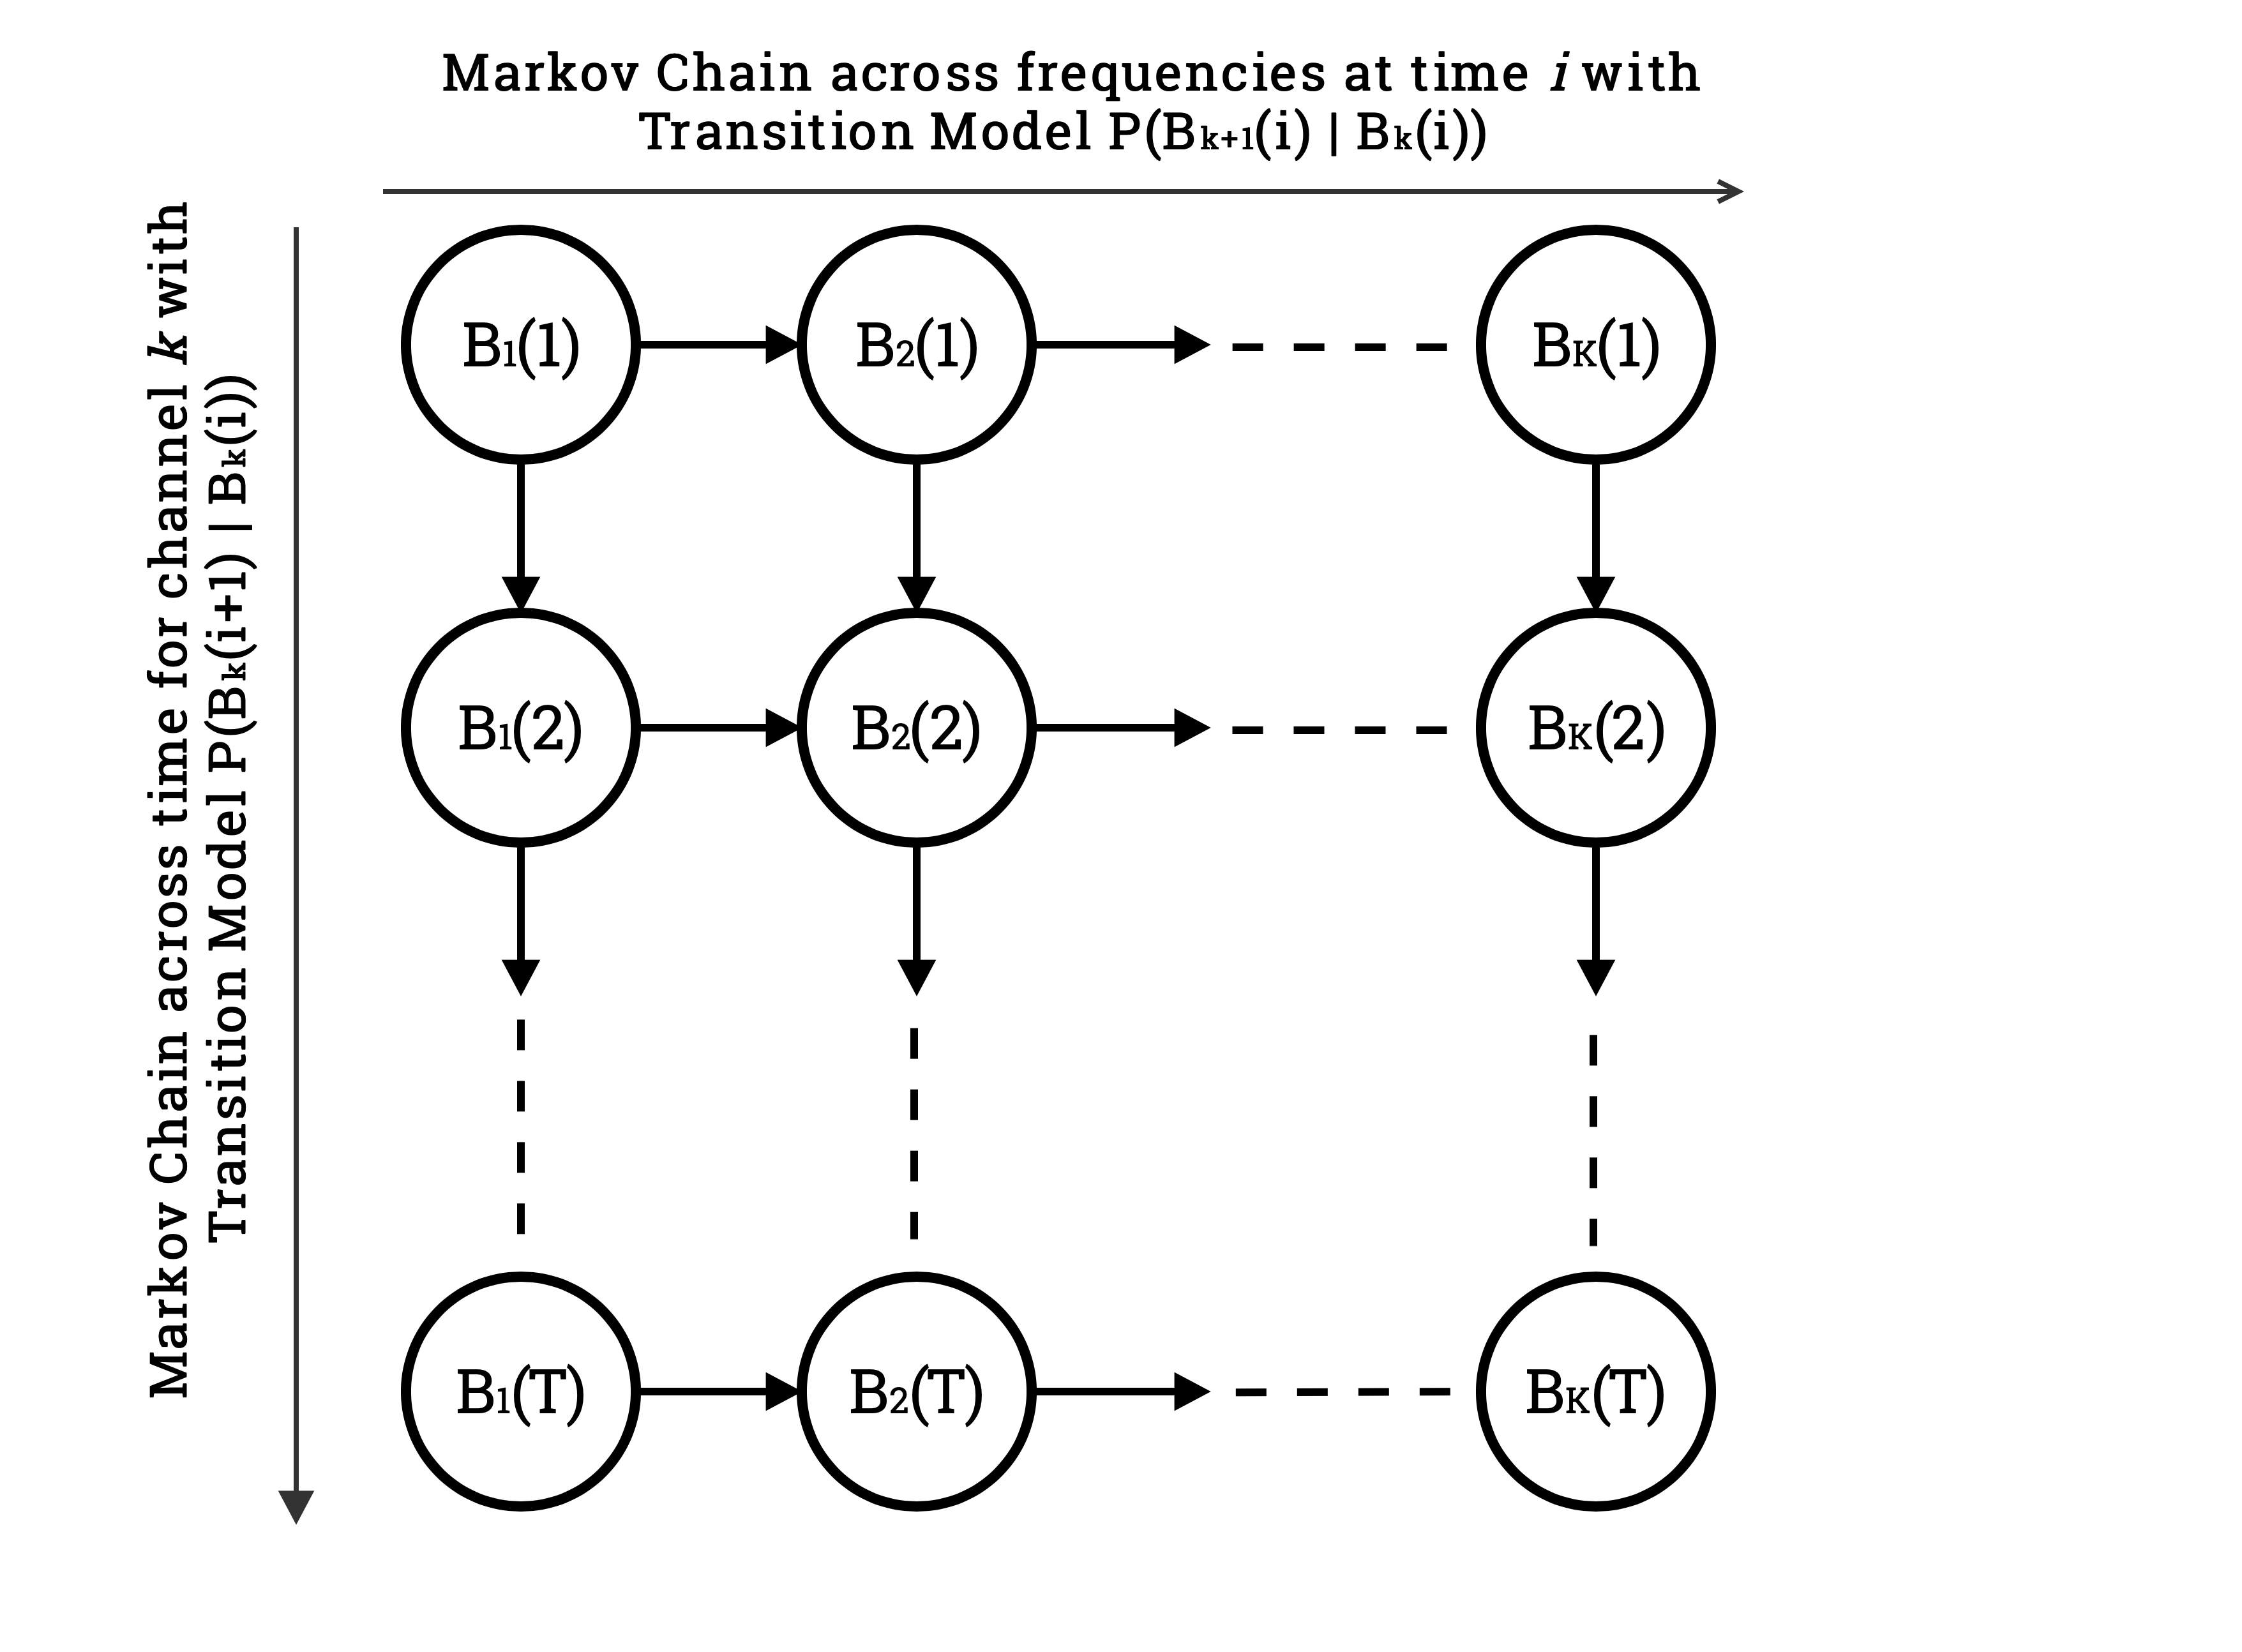
\includegraphics[width = 0.65\textwidth]{MarkovChainsVisualization.png}
    \caption{The \textcolor{magenta}{time-frequency correlation structure} of the incumbent occupancy behavior}
    \label{fig:31}
\end{figure}
\end{frame}
\begin{frame}{SU Spectrum Sensing Model\footnote{\tiny{S. Malecki, et. al., ``Energy and throughput efficient strategies...", 2011 IEEE 12th International Workshop on Signal Processing Advances in Wireless Communications}}}
    \begin{itemize}
        \item SU can sense \textcolor{magenta}{at most $\kappa$ out of $K$ spectrum bands at any given time}, with $1{\leq}\kappa{\leq}K$
        \item HMM framework:
        \[\vec{Y}(i) = [Y_k(i)]_{k {\in} \mathcal K_i}\text{ is the observation vector};\]
        \[f(\vec{Y}(i)|\vec{B}(i), \mathcal K_i) = \prod_{k \in \mathcal K_i} f(Y_k(i)|B_k(i))\text{ is its PDF;}\]
        \[Y_k(i)|B_k(i) \sim \mathcal{CN}(0, \sigma_H^2P_{tx}B_k(i) + \sigma_V^2)\text{ from the signal model}\]
    \end{itemize}
\end{frame}
\begin{frame}{POMDP Agent Model (1/2)}
   \begin{figure}
    \centering
    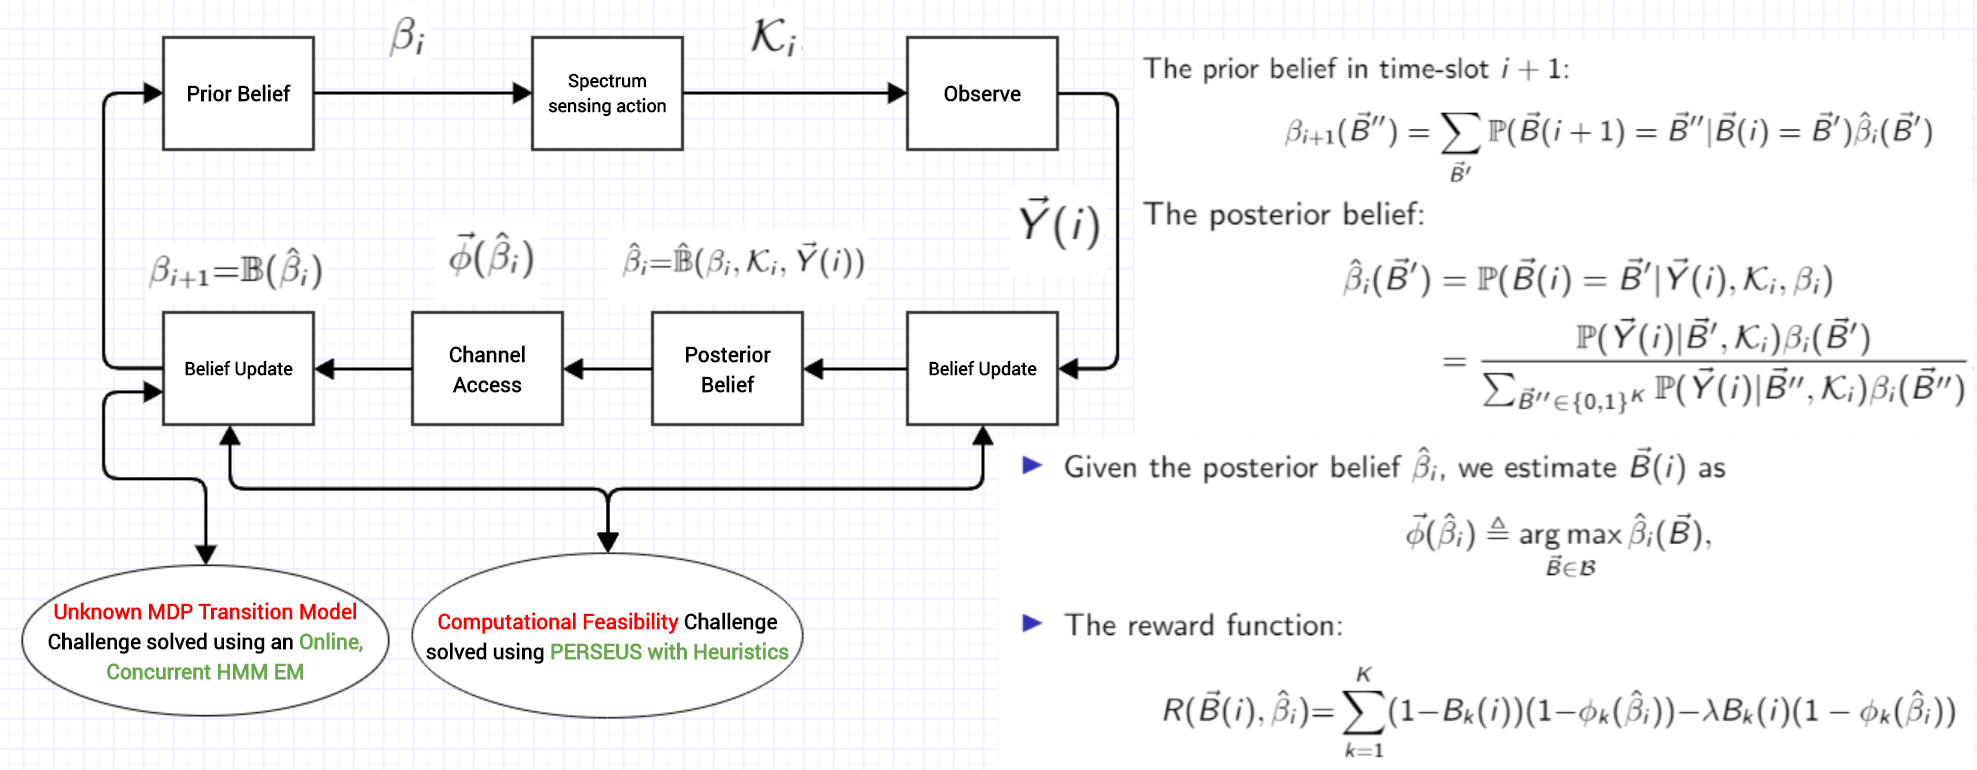
\includegraphics[width = 1.05\textwidth]{POMDP_Final.PNG}
    \caption{The POMDP Formulation}
    \label{fig:31}
\end{figure}
\end{frame}
\begin{frame}{POMDP Agent Model (2/2)}
    \footnotesize{\begin{itemize}
        \item Exploit the Markovian correlation model\footnote{\tiny{S. Mosleh, et. al., ``Performance analysis of the Neyman-Pearson fusion center...", IEEE EUROCON 2009}}
        \item \textcolor{magenta}{Goal}: Find optimal spectrum sensing policy that maximizes the infinite-horizon discounted reward:
        \[\pi^{*}{=}\argmax_{\pi} V^{\pi}(\beta) \triangleq \mathbb{E}_{\pi} \Big[\sum_{i=1}^{\infty} \gamma^{i} R(\vec{B}(i), \hat{\beta}_i)|\beta_0 {=}\beta\Big]\]
        \item $\pi^{*}$ is the solution to $V^*{=}\mathcal{H}[V^*]$; \textcolor{magenta}{Bellman operator} $V_{t+1}{=}\mathcal {H}[V_{t}]$ is
        \[V_{t+1}(\beta) = \max_{\mathcal{K} {\in} \mathcal{A}} \sum_{\vec{B} {\in} \mathcal{B}} \beta(\vec{B}) \mathbb{E}_{\vec{Y}|\vec{B}, \mathcal{K}} \Big[R(\vec{B}, \hat{\mathbb{B}}(\beta, \mathcal{K}, \vec{Y}))+\gamma V_{t}(\mathbb{B}(\hat{\mathbb{B}}(\beta, \mathcal{K}, \vec{Y})))\Big],\ \forall \beta\]
    \end{itemize}}
\end{frame}
\begin{frame}{The Parameter Estimator\footnote{\tiny{W. Turin, ``Map decoding using the EM algorithm", 1999 IEEE 49th Vehicular Technology Conference}}}
    \begin{itemize}
        \item MLE problem:
        \[\vec{\theta}^{*} = \argmax_{\vec{\theta}} \log\Big(\sum_{\mathbf{B}} \mathbb{P}(\mathbf{B}, \mathbf{Y}| \vec{\theta})\Big)\]
        \item The Baum-Welch algorithm (EM for HMMs):
        \[\text{\textcolor{magenta}{E-step}: }Q(\vec{\theta}|\vec{\theta}^{(t)}) = \mathbb{E}_{\mathbf{B}|\mathbf{Y}, \vec{\theta}^{(t)}} \Big[ \log \Big(\mathbb{P}(\mathbf{B}, \mathbf{Y}|\vec{\theta}^{(t)})\Big)\Big]\]
        \[\text{\textcolor{magenta}{M-step}: }\vec{\theta}^{(t+1)} = \argmax_{\vec{\theta}} Q(\vec{\theta}|\vec{\theta}^{(t)})\]
    \end{itemize}
\end{frame}
\begin{frame}{PERSEUS\footnote{\tiny{T.J. Spaan, et. al., ``Perseus: Randomized Point-based Value Iteration for POMDPs", Journal of Artificial Intelligence Research, 2005}} (1/2)}
\begin{itemize}
        \item \textcolor{magenta}{Initial exploration}: $\tilde{\mathcal{B}}$
        \item \textcolor{magenta}{Goal}: Improve the value of all the belief points in $\tilde{\mathcal{B}}$ by updating the value of only a subset of these belief points, chosen iteratively at random
        \item \[V_{t}(\beta) \approx \beta \cdot \vec{\alpha}_{t}^{u^*},\ u^* = \argmax_{u\in\{1,2,\dots,|\tilde{\mathcal{B}}|\}} \beta \cdot \vec{\alpha}_{t}^{u},\ \beta\cdot\vec{\alpha}{=}\sum_{\vec{B}}\beta(\vec{B})\vec{\alpha}(\vec{B})\]
\end{itemize}
\end{frame}
\begin{frame}{PERSEUS (2/2)}
    \begin{itemize}
        \item \textcolor{magenta}{Initialization}: $\tilde{\mathcal{U}}{=}\tilde{\mathcal{B}}$
        \item \textcolor{magenta}{Backup}: 
        \begin{itemize}
            \item Find a new hyperplane associated with randomly chosen $\beta_{u}$:
            \[\vec{\alpha}_{t+1}^{u}=\Xi_{\mathcal K_{t+1}^{u}}^{u},\ \mathcal K_{t+1}^{u}=\argmax_{\mathcal{K} \in \mathcal{A}} \beta_u \cdot \Xi_{\mathcal{K}}^{u}\]
            \begin{align*}
                \Xi_{\mathcal{K}}^{u}(\vec{B}) = \mathbb{E}_{\vec{Y}|\vec{B}, \mathcal{K}} \Big[&R(\vec{B}, \hat{\mathbb{B}}(\beta_{u}, \mathcal{K}, \vec{Y}))+\\&\gamma \sum_{\vec{B}'}\mathbb{P}(\vec{B}(i+1){=} \vec{B}'|\vec{B}(i){=}\vec{B})\Xi_{\mathcal{K}, \vec{Y}}^{u}(\vec{B}')\Big]
            \end{align*}
            \[\scriptsize{\text{Future value function: }}\Xi_{\mathcal{K}, \vec{Y}}^{u}=\argmax_{\alpha_{t}^{u'}, u' {\in} \{1, 2, \dots, |\tilde{\mathcal{B}}|\}} \mathbb{B}(\hat{\mathbb{B}}(\beta_{u}, \mathcal{K}, \vec{Y}))\cdot\alpha_{t}^{u'}\]
            \item $$
                    \tilde{\mathcal{U}}\leftarrow \tilde{\mathcal{U}}\setminus\{\beta_u\}\setminus
                    \{\beta'\in\tilde{\mathcal{U}}:\beta'{\cdot}\vec{\alpha}_{t+1}^{u}\geq V_t(\beta')\}
                 $$
            \item \textcolor{red}{Backup termination}: $\tilde{U}{=}\phi$
        \end{itemize}
        \item \textcolor{red}{PERSEUS Termination}: $|V_{t{+}1}(\beta){-}V_{t}(\beta)|{<}\epsilon,\ \forall \beta{\in} \tilde{\mathcal{B}},\ \epsilon{>}0$
    \end{itemize}
\end{frame}
\begin{frame}{PERSEUS Heuristics}
    \begin{itemize}
        \item \textcolor{cyan}{Fragmentation}: smaller, independent sets of correlated channels governed by incumbent-specific behavior
        \item \textcolor{cyan}{Belief Update Simplification}: Hamming distance filter to avoid iterating over all possible states
    \end{itemize}
\end{frame}
\begin{frame}{Simulation setup}
   \footnotesize{\begin{itemize}
        \item $\vec{p}{=}[p_{00}{=}0.1,p_{01}{=}p_{10}{=}0.3,p_{11}{=}0.7]^\intercal$ and $\vec{q}{=}[q_{0}{=}0.3,q_{1}{=}0.8]^\intercal$
        \item $\kappa{=}6$
        \item 
        $$C^{\text{SU}} = \frac{1}{T}\sum_{i=1}^T \sum_{k=1}^{K} R_{\text{SU}} \cdot \mathcal{I}\left(\text{SINR}_{\text{SU}}(k,i) \geq 2^{R_{\text{SU}}/\text{BW}} - 1\right),$$ $R_{\text{SU}}{=}0.6$Mbps
        \item
        $$C^{\text{PUs}}{=}\frac{\sum_{i=1}^{T}\sum_{k=1}^{K}R_{\text{PU}}B_{k}(i)\mathcal{I}\left(\text{SINR}_{\text{PU}}(k,i){\geq}2^{R_{\text{PU}}/\text{BW}}{-}1\right)}{\sum_{i=1}^T\sum_{k=1}^{K}B_{k}(i)},$$
        $R_{\text{PU}}{=}0.9$Mbps
        \item $\gamma{=}0.9$, $\epsilon{=}10^{-5}$, Hamming distance filter metric${=}3$
    \end{itemize}}
\end{frame}
\begin{frame}{Numerical Evaluations (1/6)}
    \begin{figure}
    \centering
    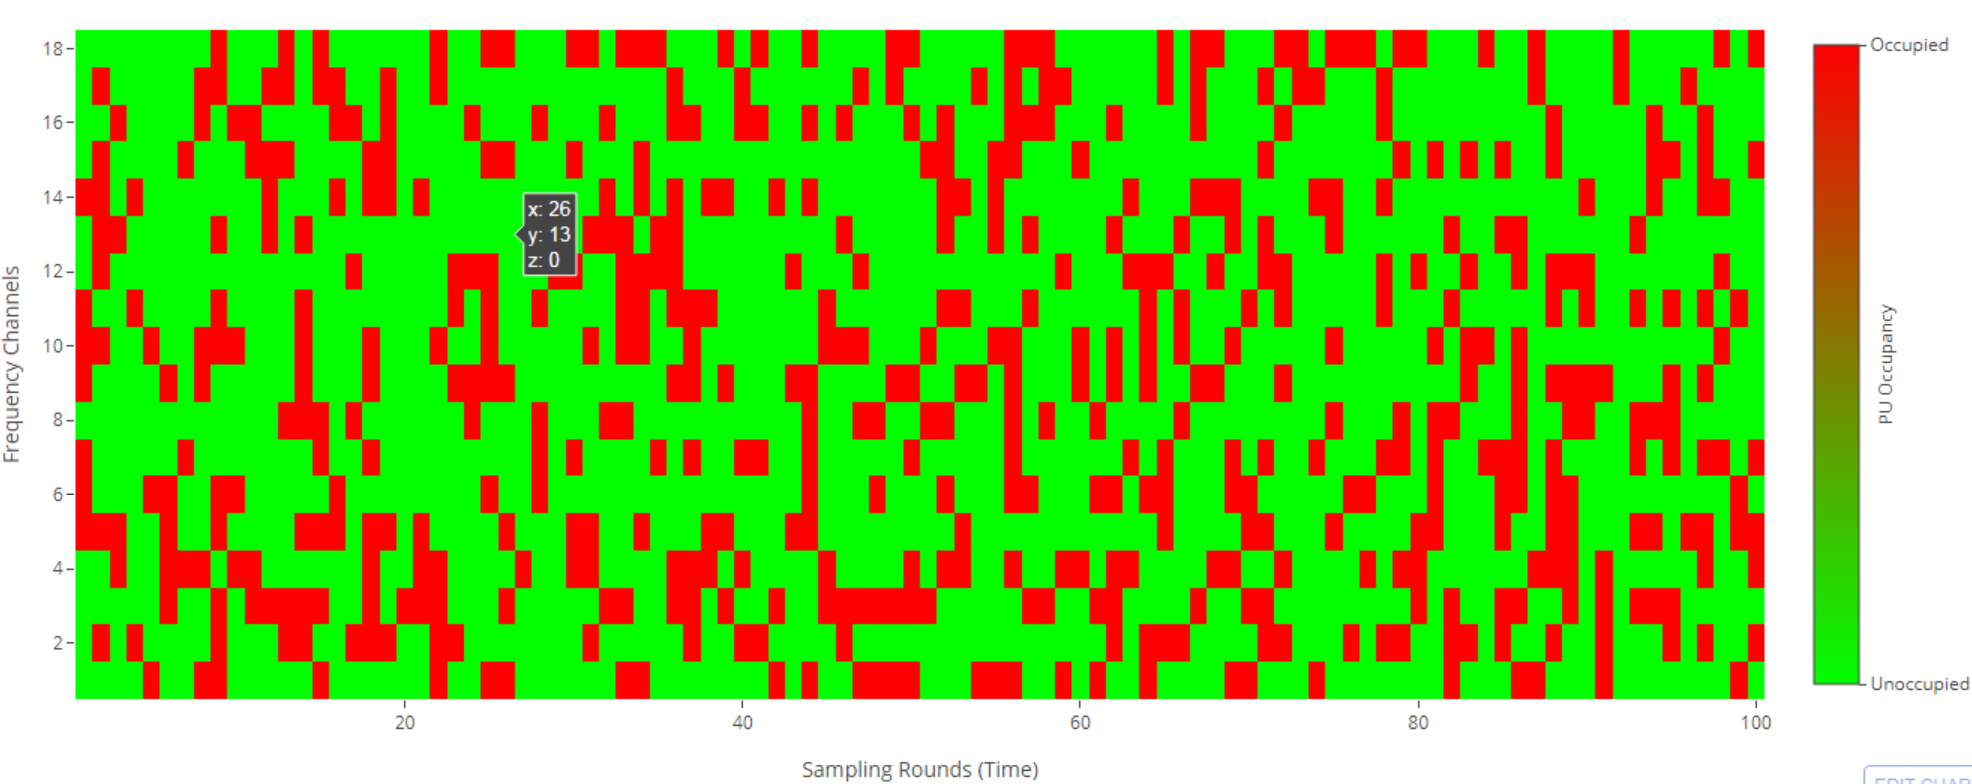
\includegraphics[width = 1.0\textwidth]{Independence_1.PNG}
    \caption{The time-frequency incumbent occupancy behavior assuming \textcolor{magenta}{independence across both frequency and time}}
    \label{fig:29}
\end{figure}
\end{frame}
\begin{frame}{Numerical Evaluations (2/6)}
    \begin{figure}
    \centering
    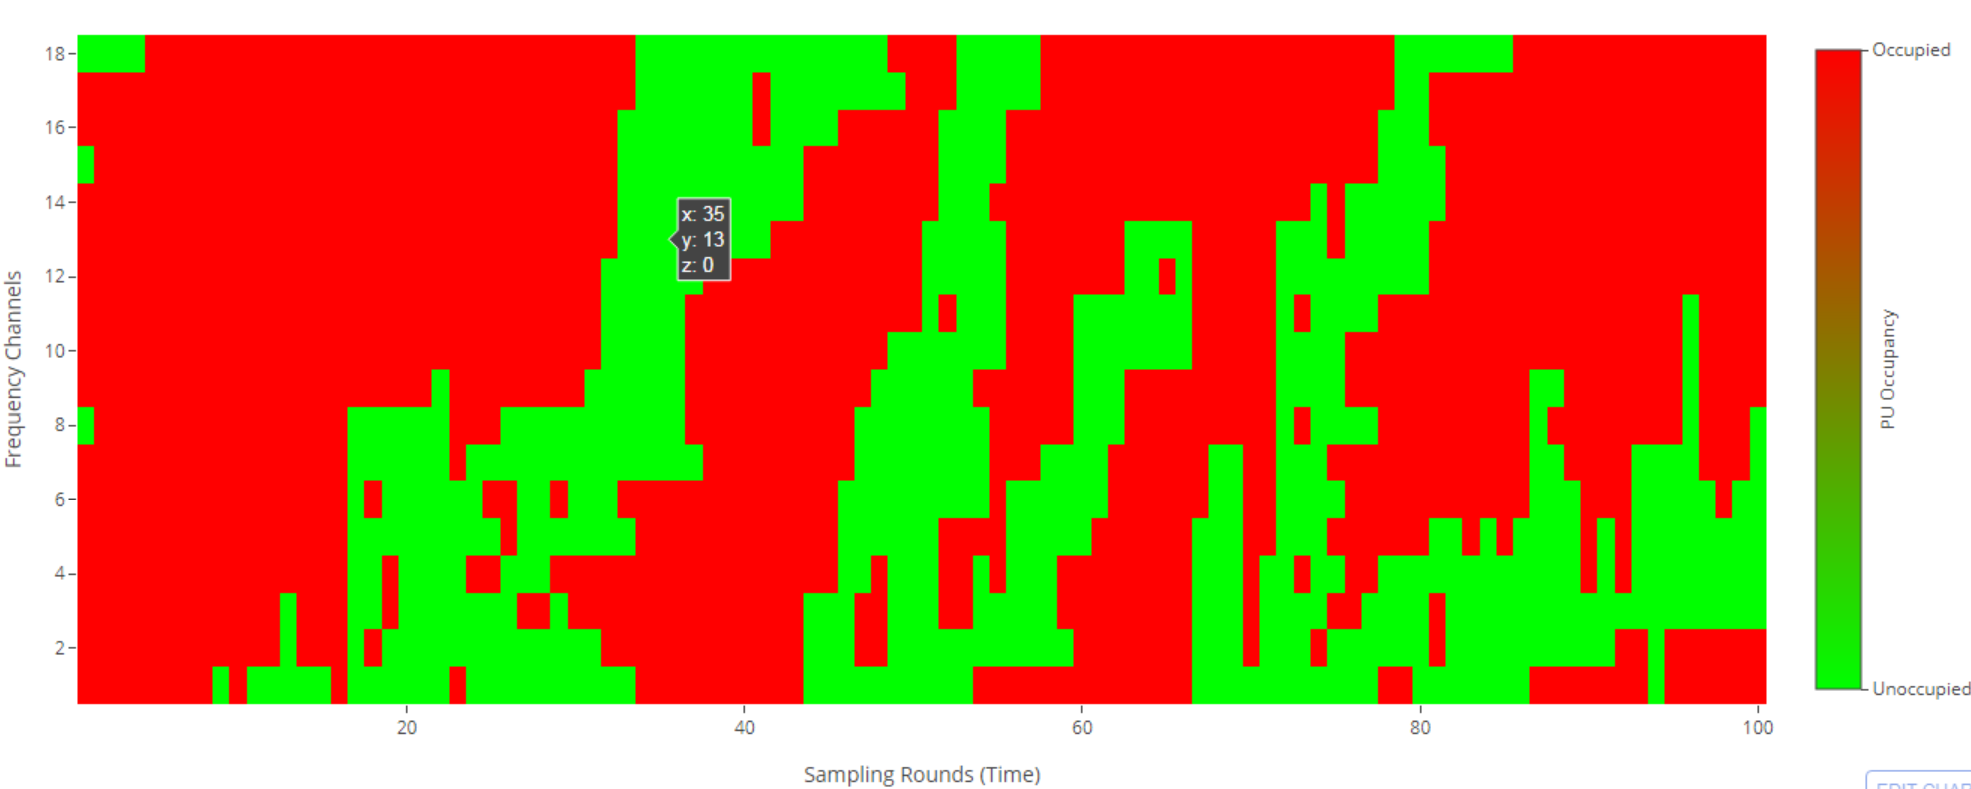
\includegraphics[width = 1.0\textwidth]{Space_Time_Corr_1.PNG}
    \caption{The time-frequency incumbent occupancy behavior assuming a \textcolor{magenta}{Markovian correlation across both frequency and time}}
    \label{fig:30}
\end{figure}
\end{frame}
\begin{frame}{Numerical Evaluations (3/6)}
    \begin{figure}
    \centering
    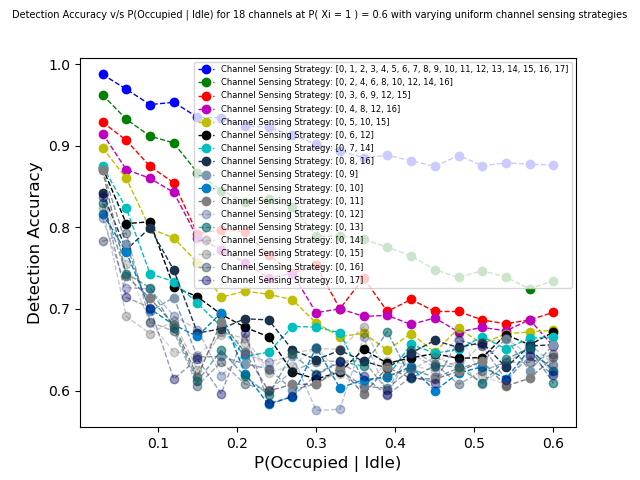
\includegraphics[width = 0.85\textwidth]{Uniform_Channel_Sensing.png}
    \caption{Single Markov chain across channels: Effect of channel \textcolor{magenta}{sensing limitations}, \textcolor{magenta}{channel correlation}, and \textcolor{magenta}{sensing strategies} on estimation/detection accuracy}
    \label{fig:32}
\end{figure}
\end{frame}
\begin{frame}{Numerical Evaluations (4/6)}
    \begin{figure}
    \centering
    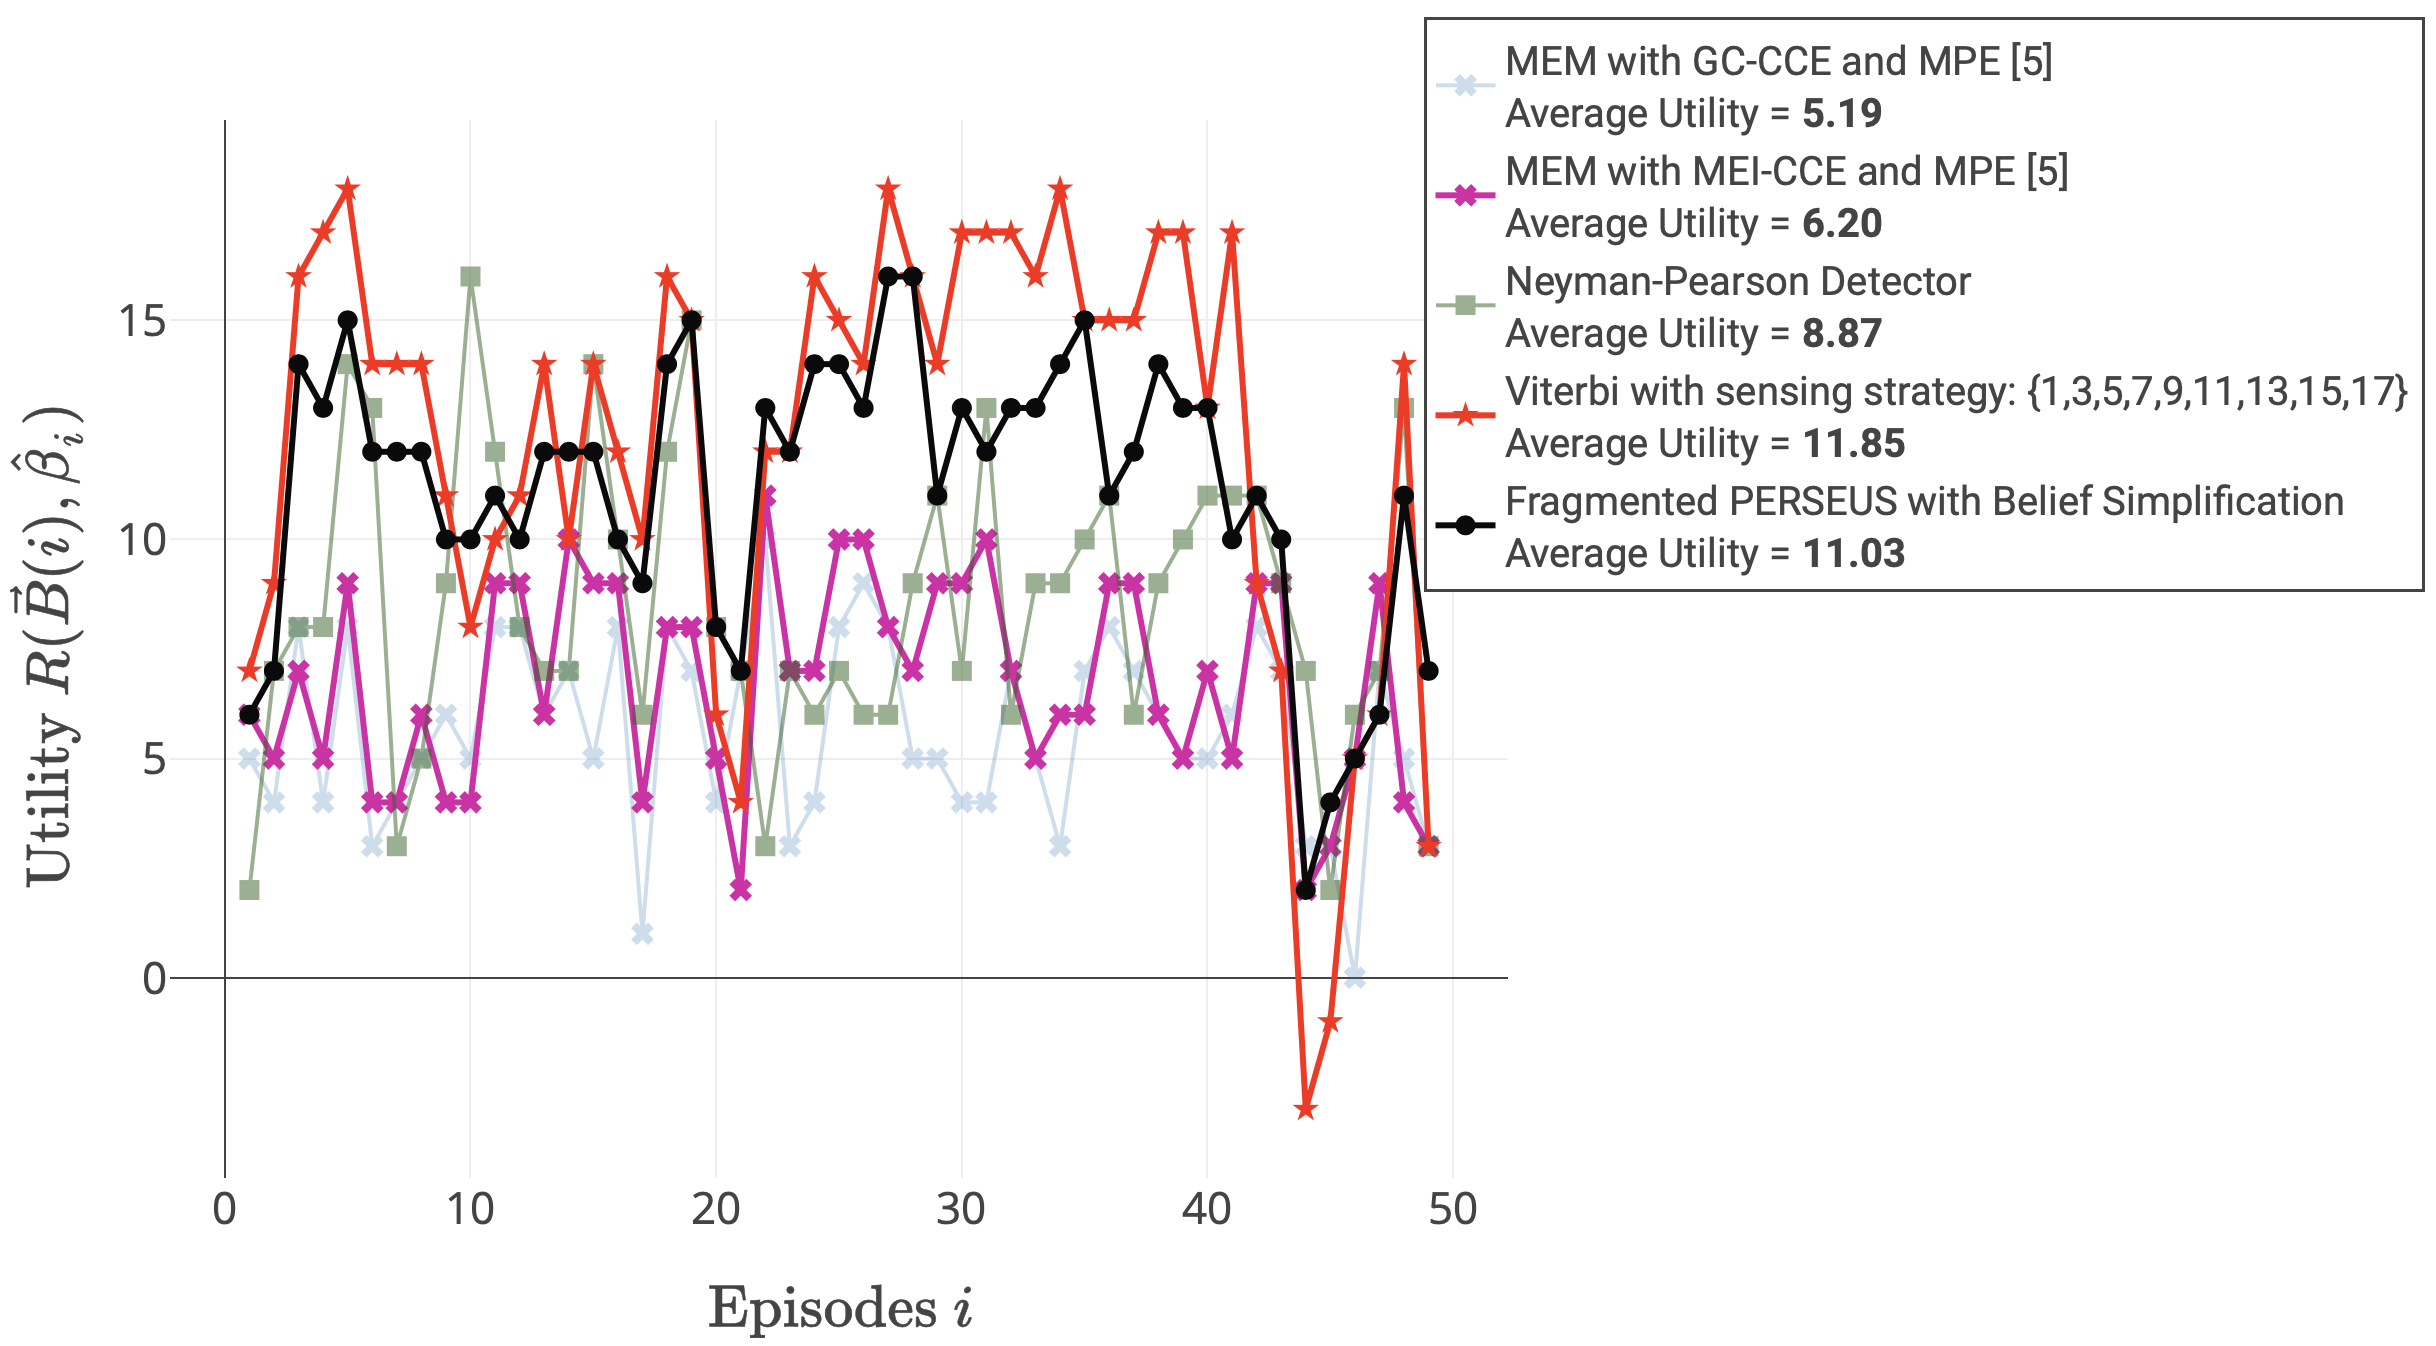
\includegraphics[width = 0.95\textwidth]{PerformanceEvaluation.png}
    \caption{The comparison of the \textcolor{magenta}{utility obtained by our framework per time-slot} against that obtained by other schemes in the state-of-the-art}
    \label{fig:33}
\end{figure}
\tiny{[5]: M. Gao, et. al., ``Fast Spectrum Sensing...", 2014 IEEE MilCom}
\\\tiny{[Viterbi]: C. Park, et. al., ``HMM Based Channel Status Predictor for Cognitive Radio", 2007 APAC MW Conf}
\\\tiny{[NPD]: S. Mosleh, et. al., ``Performance analysis of the Neyman-Pearson fusion center...", IEEE EUROCON 2009}
\end{frame}
\begin{frame}{Numerical Evaluations (5/6)}
    \begin{figure}
    \centering
    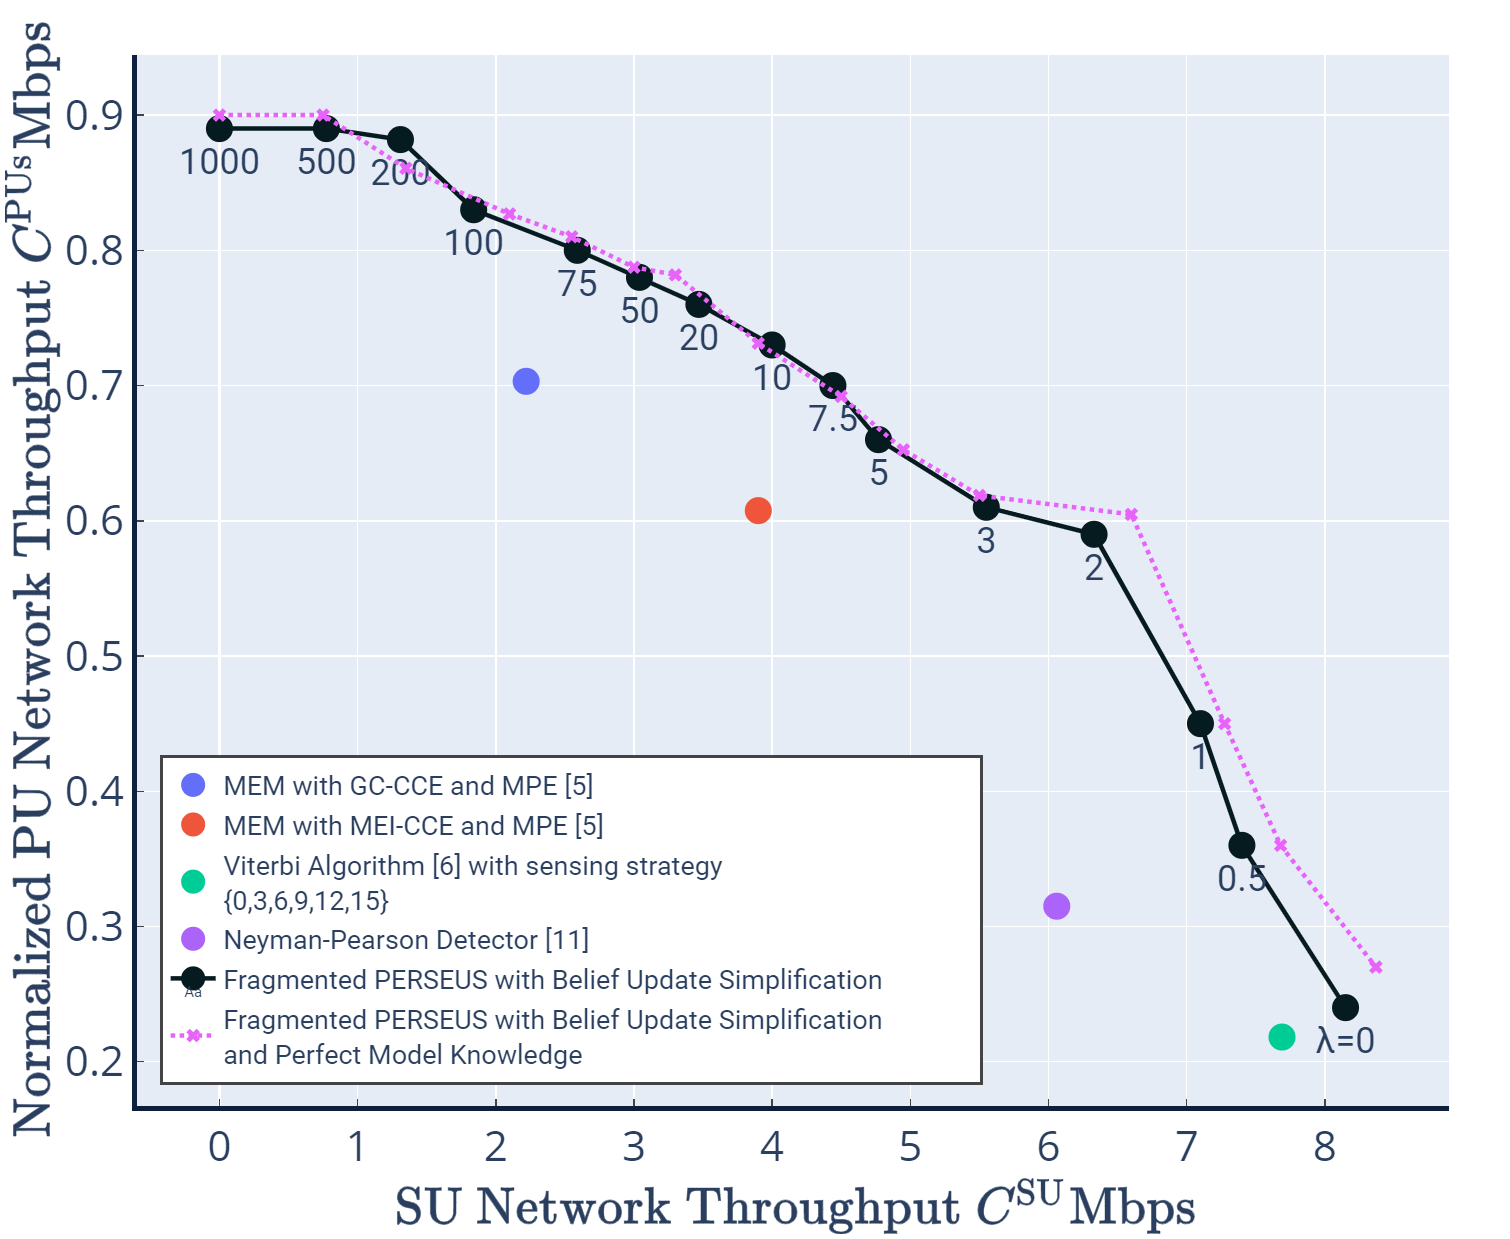
\includegraphics[width = 0.7\textwidth]{Perf_Complete.PNG}
    \caption{Evaluation of $C^{\text{SU}}$ versus $C^{\text{PUs}}$ for different values of the penalty $\lambda$; \textcolor{magenta}{comparison with state-of-the-art}}
    \label{fig:34}
\end{figure}
\tiny{[5]: M. Gao, et. al., ``Fast Spectrum Sensing...", 2014 IEEE MilCom}
\\\tiny{[6]: C. Park, et. al., ``HMM Based Channel Status Predictor for Cognitive Radio", 2007 Asia-Pacific MW Conf}
\\\tiny{[11]: S. Mosleh, et. al., ``Performance analysis of the Neyman-Pearson fusion center...", IEEE EUROCON 2009}
\end{frame}
\begin{frame}{Numerical Evaluations (6/6)}
    \begin{figure}
    \centering
    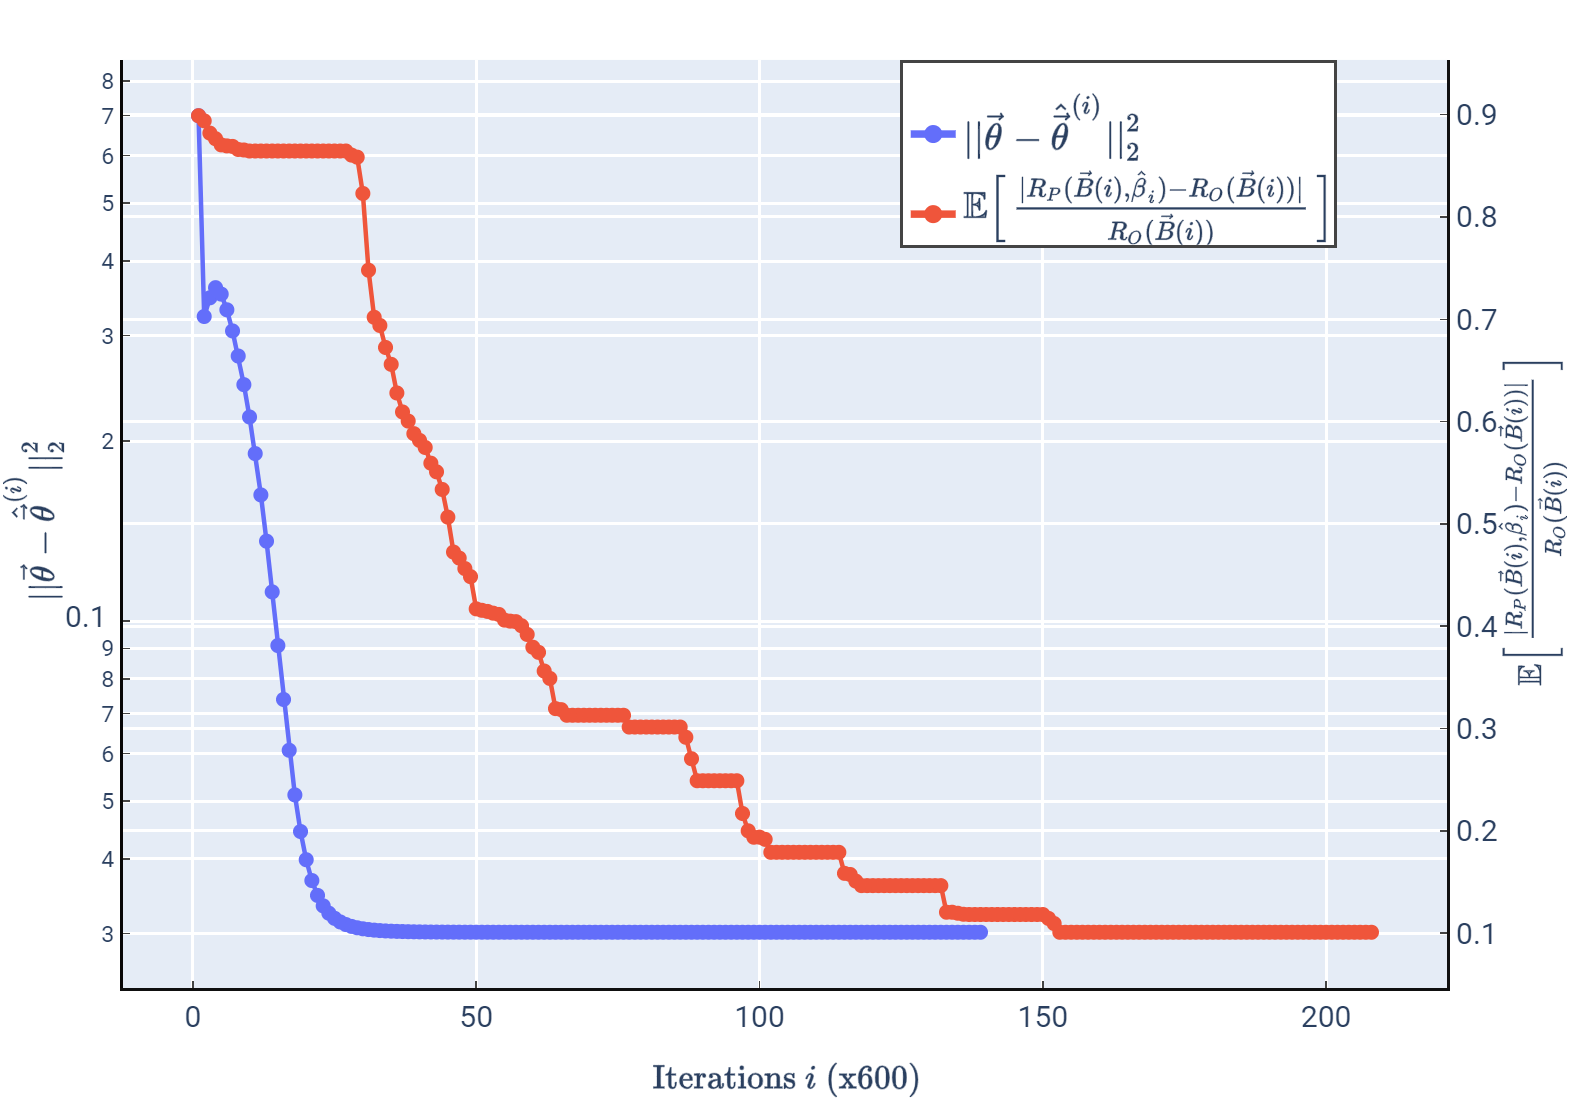
\includegraphics[width = 0.85\textwidth]{Final_Perf_2.PNG}
    \caption{Convergence of: MSE of the EM algorithm to estimate $\vec{\theta}$; and \textcolor{magenta}{Normalized sub-optimal gap} of the fragmented PERSEUS algorithm with belief update simplification}
    \label{fig:35}
\end{figure}
\end{frame}
\begin{frame}{POMDP Access Policy Implementation}
\begin{figure}
    \centering
    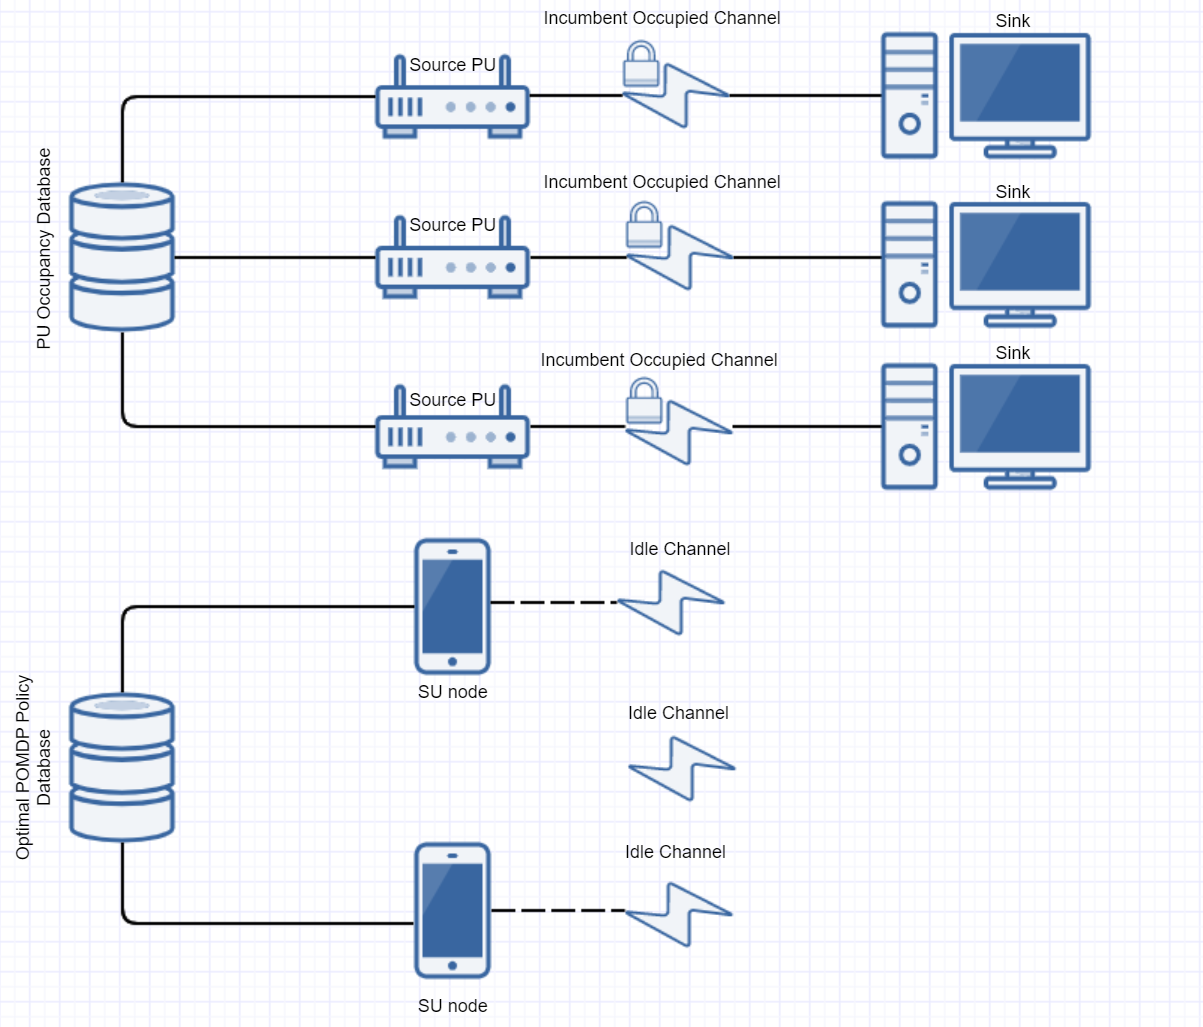
\includegraphics[width = 0.8\textwidth]{ESP32_Deployment.PNG}
    \caption{\scriptsize{The distributed ad-hoc network consisting entirely of \textcolor{magenta}{ESP$32$} radios serving as PU sources, sinks, \& SUs}}
    \label{fig:35}
\end{figure}
\end{frame}
\begin{frame}{Time-slotted Detection Accuracy\footnote{\tiny{Recent Update: Need to compare this performance with a situation where incumbent occupancy independence is assumed across time and frequency}}}
    \begin{figure}
    \centering
    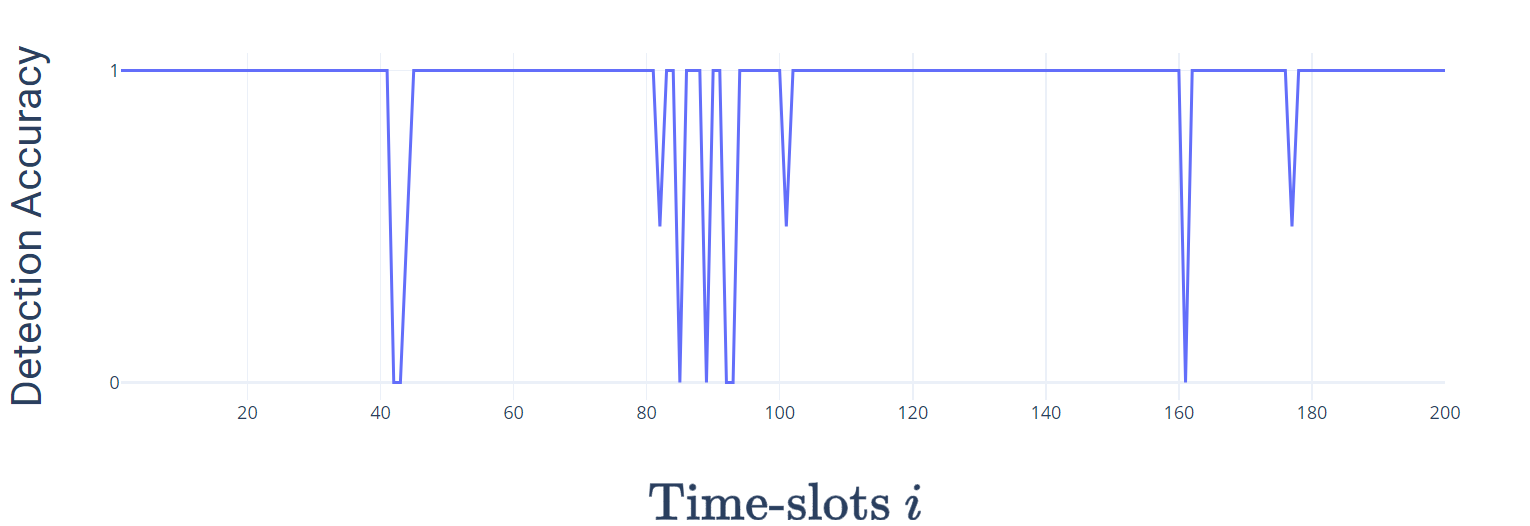
\includegraphics[width = 1.0\textwidth]{ESP32.PNG}
    \caption{The time-slotted \textcolor{magenta}{detection accuracy} of the cognitive radios (SUs) in this distributed ad-hoc network of ESP$32$ radios over $2.4$GHz WiFi channels}
    \label{fig:36}
\end{figure}
\end{frame}
\begin{frame}{}
  \centering \Huge
  \emph{Q\&A}
\end{frame}
\begin{frame}{}
  \centering \Huge
  \emph{Thank you}
\end{frame}
\end{document}